%%%%%%%%%%%%%%
% Fichero: uclmTFGesi.tex
% Autor: Jesús Salido Tercero (http://www.uclm.es/profesorado/jsalido)
% Fecha (creación): Febrero 2010 
% Rev. : Febrero 2019
% Descripción: Plantilla para memoria de TFG 
% (Escuela Sup. de Informática, UCLM). Creada para el curso 
% “LaTeX esencial para preparación de TFG, Tesis y otros documentos 
% académicos” (Esc. Sup. Informática-UCLM)
%
% Comentarios: Preparada para `pdflatex' y `biblatex' (con `biber'). 
% Documento editado con TeXstudio. 
% Para su compilación se aconseja utilizar latexmk y biber (requiere perl):
% $latexmk -pdf -silent -synctex=1 --enable-write18 % (última opción innecesaria en Unix)
% En sistemas Unix: latexmk y biber deben ser instalados por separado.
%
% Una versión actualizada de esta plantilla está disponible en overleaf.
% Puede crearse un proyecto propio para escribir un TFG directamente en overleaf,
% o bien descargarla como un archivo .zip para su utilización en modo local.
%%%%%%%%%%%%%%


% -------------------------
%
% PREÁMBULO del documento
% (Editar sólo en caso de cambio del idioma pral. del documento u
%  opciones de los paquetes incluidos).
%
% -------------------------
% EDITAR: Idioma pral. \spanishtrue (Español), \spanishfalse (Inglés)
%Comentar opción no deseada
\newif\ifspanish%Definición de un condicional (spanish)

\spanishtrue 			% Idioma pral.: español (spanish=true)
%\spanishfalse			% Idioma pral.: inglés (spanish=false)
	
\documentclass[ 		% Clase del documento
	11pt,				% Tamaño de letra
	a4paper,			% Tamaño de papel
	twoside,			% Impresión a doble cara
	openright,			% La apertura de cap. a la dcha.
	final       		% Versión final
]{book}

\usepackage[utf8]{inputenx} % Codificación de entrada
\usepackage[english,spanish,es-tabla,es-noindentfirst]{babel} % Internacionalización
%\usepackage{indentfirst} % Para asegurar sangrado en 1ª línea tras sección (necesario con varios idiomas)
\usepackage{multirow}

%--- Geometría de las páginas del documento
\usepackage[			% Márgenes del documento
	top=2.5cm,			% Margen superior
	bottom=2.5cm,		% Margen inferior
	inner=3.5cm,		% Margen al interior
	outer=2cm			% Margen al exterior
]{geometry}


%--- Tipografía
\usepackage{textcomp,marvosym,pifont} % Generación de símbolos especiales
\usepackage{ccicons} % Iconos de licencia Creative Commons
\usepackage{amsmath,amsthm,amssymb}	% Mejoras cuando hay matemáticas


%--- Tipografía (Opción 1)
\usepackage[tt=false]{libertine}	% Libertine
\usepackage[libertine]{newtxmath}	% Times
%---


%--- Tipografía (Opción 2)
%\usepackage{newpxtext}				% Palatino: La opción osf proporciona números en old style.
%\usepackage{newpxmath}				% Palatino
%---


\usepackage[T1]{fontenc}% Codificación de salida    
\usepackage{microtype}	% Mejoras de microtipografía en la obtención de PDF (sólo para pdflatex)


\usepackage{url} 		% Para escritura de URL
\urlstyle{sf}			% Estilo sans serif para URLs


%--- Definición de colores
% Este paquete debe cargarse antes de ctable.
% Revisar la documentación del paquete para ver los nombres de colores predefinidos.
\usepackage[%
	usenames,
	dvipsnames,
	svgnames,
	x11names,
	table
]{xcolor}


%--- Color especial definido para los hiperenlaces
\definecolor{palered}{rgb}{.8,0,0}


%--- Generación de hiperenlaces
\usepackage[
	pdftex,
	breaklinks,			% Permite que los links ocupen más de una línea
%	hidelinks,			% Oculta el color y borde de los links
% OJO: La opción colorlinks se comenta para evitar un error con el paquete menukeys. 
%	colorlinks=true,	% Pone color en los link o un borde
	linkcolor=palered,	% Color de los links
	anchorcolor=palered, 
	citecolor=palered, 
	filecolor=palered, 
	menucolor=palered, 
	urlcolor=palered,
	bookmarksnumbered=true % Incluye números en bookmarks
]{hyperref}


\usepackage{pdfpages}  % Permite inclusión de páginas de un PDF


%--- Paquetes para listas y organización de texto
\usepackage{paralist}	% Mayor control de listas
\usepackage{multicol}	% Texto en varias columnas


%--- Gráficos y tablas
\usepackage{graphicx}	% Inclusión de figuras
\usepackage{subfigure}	% Inclusión de subfiguras
% EDITAR: Si es necesario cambiar el path para los directorios de figuras.
\graphicspath{{./figs/}}% Path de búsqueda de ficheros gráficos
\DeclareGraphicsExtensions{.pdf,.png,.jpg} % Precedencia de extensiones
\usepackage{rotating}	% Giro de cajas (texto, figuras, tablas) (No DVI)
\usepackage{tabularx,booktabs}	% Ajustes para tablas


%--- Paquetes especiales para Informática
\usepackage{listings}	% Inclusión de listados de código

% Inclusión de algoritmos
\usepackage[
	lined,
	boxruled,
	algochapter,
	commentsnumbered,
\ifspanish
	spanish
\else
	english
\fi
]{algorithm2e}



%--- Personalización de títulos de figuras y tablas
\usepackage[%
	margin=10pt,		% Margen
	font=small,			% Tamaño de tipografía
	labelfont=bf,		% Prefijo-Etiqueta en negrita
	format=hang			%
]{caption}
\captionsetup[table]{skip=4pt} 	% Separación del caption en las tablas


%--- Bibliografía: Biblatex con biber.
% OJO: Para bib multilingüe añadir campos language y langid en registros bib.
\usepackage[
	backend=biber, 		% Backend
	sortcites,
	defernumbers=true, 	% Para numerar al final
	style=numeric-comp, % Estilo numérico condensado
	% Descomentar las opciones siguientes para bibliografía multilingüe
%	autolang=other, 	% Requerido para opción multilingüe
%	language=auto   	% Requerido para opción multilingüe
]{biblatex}


% Línea añadida para eliminar el idioma de la fuente bibliográfica.
\AtEveryBibitem{\clearfield{note} \clearlist{language}}
% OJO: Editar si se cambia el fichero de bibliografía. 
\addbibresource{biblioTFG.bib} 	% Fichero de bibliografía.
\usepackage[autostyle]{csquotes}
%---



%--- Paquete con personalización local para el TFG (ESI-UCLM)
\usepackage{uclmTFGesi}
% -------------------------
% PAQUETES QUE USA: 
% 	fancyhdr,titlesec,sectsty,tikz
% -------------------------
% LISTA DE COMANDOS PROPORCIONADOS:
% OB-Obligatorio
% OP-Opcional
% RE-Recomendado
%
% Comandos para definir variables con los datos del documento.
%
% OB-\portadaTFG				: Pág. de portada (usa variables definidas)
% OB-\portadillaTFG				: Pág. de portada interna
% OB-\tribunalTFG				: Pág. tribunal
% RE-\dedicado{texto}			: Pág. de dedicatoria con texto
% RE-\creditos{texto}{imagen}	: Pág. de créditos con el texto y la imagen
% OB-\abstract{texto}			: Añade abstract (no definido en clase book)
% OP-\tecla{texto}				: Borde de tecla en torno al texto (sustituir por menukeys)		
% OP-\nodivide[penalty]			: Penaliza la división de palabras. 
%								  Máx. (n=10000) sin arg.
% OP-\nowidowandorphan[penalty]: Penaliza las viudas y huérfanas.
%								(sólo si necesario)
% OP-\nodividenotes[penalty]	: Penaliza la división de notas al pié 
%								entre págs.	(sólo si necesario)	
% OP-\savepagecnt				: Crea contador interno con el nº de pág. actual
% OP-\contpagination			: Recupera el valor de pág. previamente
%								 salvado en el cont. interno.
% RE-\cleanhdfirst				: Elimina la cabecera en la primera 
%								página de capítulo.
%
% -------------------------




%--- Paquete para índice temático
\usepackage{makeidx}
\makeindex


%--- Paquete para incluir menús, paths y teclas de modo "elegante"
% OJO: Este paquete presenta algunas incompatibilidades, debe cargarse el último y exige la desactivación de la opción colorlinks y la inclusión en este paquete de la opción hyperrefcolorlinks.
% Este paquete presenta alguna incompatibilidades por lo que cambiarlo de ubicación puede generar algún error (manejar con cuidado).
\usepackage[os=win,hyperrefcolorlinks]{menukeys}

% Estas definiciones permiten cambiar el estilo de los elementos. Si se desean otros estilos o su configuación es preciso recurrir a la documentación del paquete (no lo recomiendo).
\renewmenumacro{\menu}[>]{menus} % default: menus
\renewmenumacro{\directory}[/]{pathswithblackfolder} % default: paths
\renewmenumacro{\keys}[+]{shadowedroundedkeys} % default: roundedkeys

%%%%%%%%%%%%%%%%%%%%%%%%%%%%%%%%%%%%%%%%%%%%%%%%%%%%%
%%%%%%%%%%%%%%%%%%%%%%%%%%%%%%%%%%%%%%%%%%%%%%%%%%%%%
%%%%%%%%%%%%%%%%%%%%%%%%%%%%%%%%%%%%%%%%%%%%%%%%%%%%%





% -------------------------
%
% DATOS DEL DOCUMENTO 
% Definición de variables empleadas en el documento por lo que no son
% traducidos. Cuando algún campo puede tener varias líneas aparecen dos
% campos señalados como <campo>Primera y <campo>Segunda.
% Si no se desea emplear un campo este debe comentarse.
%
% -------------------------
% EDITAR: Datos del documento
\tituloPrimera{Plantilla de TFG para ESI-UCLM}	% 1ª Línea
\tituloSegunda{Curso de {\LaTeX{}} esencial}			% 2ª Línea  % Comentar si no existe
\titulo{Plantilla TFG}							% Título corto
\autor{Jesús Salido Tercero}
\email{jesus.salido@uclm.es}					
\director{<director (nombre apellidos)>}
\codirector{<codirector (nombre apellidos)>}	% Comentar si no existe
\instEdu{UNIVERSIDAD DE CASTILLA-LA MANCHA}
% Fichero con escudo de la institución
% Poner el logo del centro que corresponda
%\escudo{esi} 								
%\escudo{esicolor} 
%\escudo{logo_ESI} 							
\escudo{escudoInf} 	% Nucleo de ferrita						
%\escudo{uclm} 
%\escudo{etsii} 

\centroEdu{ESCUELA SUPERIOR DE INFORMÁTICA}
\deptoEduPrimera{<Primera línea Depto. Director>}% 1ª Línea
\deptoEduSegunda{<Segunda línea Depto. Director>}% 2ª Línea  % Comentar si no existe
\titulacion{GRADO EN INGENIERÍA INFORMÁTICA}
\especialidad{<Tecnología Específica>} 			% Tecnología específica, ...
\tipoDoc{TRABAJO FIN DE GRADO}
% Si las fechas se desean en inglés hay que ponerlas explícitamente.
\fechaDef{<mes, año>} 							% Fecha de defensa
\mesDef{<mes>}        							% Mes de defensa
\yearDef{<año>}        							% Año de defensa
\lugarDef{Ciudad Real}							% Lugar de defensa


% --- Propiedades para el documento PDF
\hypersetup{%
% EDITAR: Valores para el PDF.	
	pdftitle={Plantilla TFG}, 	% Título
	pdfauthor={J. Salido},	% Autor
	pdfsubject={Plantilla LaTeX},	% Tema
	pdftoolbar=true,		% Muestra la toolbar de Acrobat
	pdfmenubar=true			% Muestra la menubar de Acrobat
}
% -------------------------




% -------------------------
%
% CUERPO DEL DOCUMENTO
%
% -------------------------
\begin{document}
	
%--- Ajustes del documento (en páginas iniciales).
\ifspanish
	\selectlanguage{spanish}% Emplea idioma español
\else
	\selectlanguage{english}% Emplea idioma inglés
\fi

\frontmatter
% Cambia la numeración de páginas a números romanos y las secciones no están numeradas aunque si aparecen en el índice de contenidos.
\pagestyle{empty}  % Páginas sin cabecera ni pies
%---



% -------------------------
%
% PORTADAS
%
% -------------------------
\portadaTFG		% Portada pral.

\portadillaTFG	% Portada interior (añade tutores)
%---






% -------------------------
%
% CRÉDITOS
%
% -------------------------
% EDITAR (opcional): Licencia (si se desea modificar).
% Este comando permite una gran flexibilidad y la ventaja de no depender de paquetes externos.
% Esta es una página reservada para señalar información relativa a los derechos de autor y la licencia de distribución y uso del documento. Esta página debería ser aprovechada también para informar de cualquier tipo de cesión de los derechos anteriormente citados. El autor del TFG debe tener presente que el incumplimiento de la legislación vigente en materia de protección de la propiedad intelectual es de su exclusiva responsabilidad independientemente de la cesión de derechos que este haya convenido para su obra ya que no son objeto de cesión aquellos derechos de los que no se es poseedor.

\creditos{Este documento se distribuye con licencia Creative Commons Atribución Compartir Igual 4.0. El texto completo de la licencia puede obtenerse en \url{https://creativecommons.org/licenses/by-sa/4.0/}. 
% El escudo de Informática basado en el nuclo de ferrita que acompaña la distribución de esta plantilla ha sido realizado por P.~Moya, D.~Villa e I. Díez, su inclusión debe respetar los derechos de autor y las licencias a las que se vea sometido. 

La copia y distribución de esta obra está permitida en todo el mundo, sin regalías y por cualquier medio, siempre que esta nota sea preservada. Se concede permiso para copiar y distribuir traducciones de este libro desde el español original a otro idioma, siempre que la traducción sea aprobada por el autor del libro y tanto el aviso de copyright como esta nota de permiso, sean preservados en todas las copias.}{cclicense}
%---




% -------------------------
%
% TRIBUNAL
%
% -------------------------
\tribunalTFG % Página para calificaciones del tribunal
%---





% -------------------------
%
% DEDICATORIA (opcional, 1 pág. máximo)
% Aunque opcional, no se debería perder la oportunidad de poder 
% dedicar el trabajo a alguien MUY especial.
%
% -------------------------
% EDITAR: Dedicatoria (comentar si no se desea incluir).
\dedicado{A mis alumnos ... \\ % A alguien muy especial
(para siempre)} % Como mucho dos líneas (no confundir con los agradecimientos).
%---









%--- Ajustes del documento.
\pagestyle{plain}	% Páginas sólo con numeración inferior al pie

% -------------------------
%
% RESUMEN:
% OJO: Si es preciso cambiar orden manualmente
%
% -------------------------
%--- Resumen en español
\selectlanguage{spanish} % Selección de idioma del resumen.
\cleardoublepage % Se incluye para modificar el contador de página antes de añadir bookmark
\phantomsection  % OJO: Necesario con hyperref
\pdfbookmark[0]{Resumen}{idx_resumen}% idx_resumen.0 % Bookmark en PDF


\begin{abstract}
% EDITAR: Resumen (máx. 1 pág.)
\begin{center}
\emph{(... versión del resumen en español ...)}
\end{center}
El resumen debe ocupar como máximo una página y en dicho espacio proporcionará información crucial sobre el \emph{`qué'} (problemática que trata de resolver el TFG), el \emph{`cómo'} (metodología para llegar a los resultados) y los objetivos alcanzados.
\end{abstract}
%---










%--- Resumen en inglés
% Abstract
\selectlanguage{english} % Selección de idioma del resumen.
\cleardoublepage
\phantomsection % OJO: Necesario con hyperref
\pdfbookmark[0]{Abstract}{idx_abstract}% idx_abstract.0 % Bookmark en PDF

\begin{abstract}
% EDITAR: Abstract (máx. 1 pág.)

\begin{center}
\emph{(... english version of the abstract ...)}
\end{center}
Versión del resumen en inglés. En los trabajos cuyo idioma principal sea el inglés, el orden de \textsf{Resumen} y \textsf{Abstract} se invertirá.	
\end{abstract}
%---














% Selección de idioma para el resto del documento y adaptación de títulos de sección.
% EDITAR: Sólo si es necesario.
% NOTA: Al cambiar de idioma las def. de títulos se reinician.
\ifspanish
	\selectlanguage{spanish}% Para el resto del documento el idioma es español.
	%--- No necesarios al añadir la opción es-tabla para babel.
	%\renewcommand{\tablename}{Tabla} % Se sustituye 'Cuadro' por 'Tabla'
	%\renewcommand{\listtablename}{Índice de tablas}
	%---
	\renewcommand{\lstlistingname}{Listado}
	\renewcommand{\lstlistlistingname}{Índice de listados}
	\SetAlgorithmName{Algoritmo}{Alg}{Índice de algoritmos}
	% Modififica las macros \algorithmcfname y \listalgoritmcfname
	\renewcommand{\appendixname}{Anexo}
	\renewcommand{\bibname}{Bibliografía}
	\renewcommand{\indexname}{Índice temático}
\else
	\selectlanguage{english}
\fi

% -------------------------
%
% AGRADECIMIENTOS (recomendable máx. 1 pág.)
%
% -------------------------
\cleardoublepage
\phantomsection % OJO: Necesario con hyperref
\pdfbookmark[0]{Agradecimientos}{idx_agrad}% idx_agrad.0 % Bookmark en PDF

\chapter*{Agradecimientos} % Opción con * para que no aparezca en TOC ni numerada

%OJO: Editar
 Aunque es un apartado opcional, haremos bueno el refrán \emph{<<Es de bien nacidos, ser agradecidos>>} si empleamos este espacio es un medio para agradecer a todos los que, de un modo u otro, han hecho posible que el TFG <<llegue a buen puerto>>. Esta sección es ideal para agradecer a familiares, directores, profesores, compañeros, amigos, etc. 
 
 Estos agradecimientos pueden ser tan personales como se desee e incluir anécdotas y chascarrillos, pero nunca deberían ocupar más de una página.

\makeatletter		
\begin{flushright}
	\textit{\@autor}
\end{flushright}
\makeatother % Agradecimientos etc.












% -------------------------
%
% ÍNDICES
%
% -------------------------
\pagestyle{fancy} % Estilo de página ajustado por fancyhdr

% EDITAR: Si alguno de los índices no existe, su inclusión se puede comentar.
\cleardoublepage
\phantomsection % OJO: Necesario con hyperref
\pdfbookmark[0]{Índice general}{idx_toc}% idx_toc.0 % Bookmark en PDF

\tableofcontents  % Índice general

% Todos los listados se han incluido en el índice de contenidos. De modo automático también quedan añadidos a los bookmarks del PDF. Si se desean eliminiar del TOC se pueden comentar el comando \addcontensline.

\cleardoublepage
\phantomsection % OJO: Necesario con hyperref
\addcontentsline{toc}{chapter}{\listfigurename} % Añade la lista de figuras al TOC (también a bookmarks en PDF)
%\pdfbookmark[0]{\listfigurename}{idx_lof}% idx_lof.0 % Bookmark en PDF
\listoffigures    % Índice de figuras (opcional)

\cleardoublepage
\phantomsection % OJO: Necesario con hyperref
\addcontentsline{toc}{chapter}{\listtablename} % Añade la lista de tablas al TOC (también a bookmarks en PDF)
%\pdfbookmark[0]{\listtablename}{idx_lot}% idx_lot.0 % Bookmark en PDF
\listoftables % Índice de tablas (opcional)

\cleardoublepage
\phantomsection % OJO: Necesario con hyperref
\addcontentsline{toc}{chapter}{\lstlistlistingname} % Añade la lista de listados al TOC (también a bookmarks en PDF)
%\pdfbookmark[0]{\lstlistlistingname}{idx_lol}% idx_lol.0 % Bookmark en PDF
\lstlistoflistings % Índice de listados creados con listings (opcional)

\cleardoublepage
\phantomsection % OJO: Necesario con hyperref
\addcontentsline{toc}{chapter}{\listalgorithmcfname} % Añade la lista de algoritmos al TOC (también a bookmarks en PDF)
%\pdfbookmark[0]{\listalgorithmcfname}{idx_loa}% idx_loa.0 % Bookmark en PDF
\listofalgorithms % Índice de algoritmos creados con algortihm2e





























%--- MAINMATTER
% Capítulos del documento
% Salva en un contador interno el nº de páginas actual
% Debe ir antes de \mainmatter (antes de que se reinicie el cnt page)
\savepagecnt
\mainmatter
% Justo antes del primer capítulo del libro. Activa la numeración con números arábigos y reinicia el contador de páginas.

% OJO: No cambiar de ubicación. Elimina cabecera y pie en pág. inicial de cap.
\cleanhdfirst

% Reajuste del número de página consecutivo para no reiniciar paginación en Cáp. 1
%\contpagination % Comentado para reiniciar paginación (pag. 1)




% -------------------------
%
% CAPÍTULOS
%
% -------------------------
% Se incluye un fichero para cada capítulo. Se emplea la instrucción \include porque en los libros lo más habitual es que cada cápítulo comience en una nueva página.
%\chapter{Introducción}
\label{cap:Introduccion}

Introducción al tema, entorno y justificación de la importancia del trabajo abordado.

Estructura del resto del documento.

% ------------------------------------------------------------------------------
% Ejemplos para la plantilla
% ------------------------------------------------------------------------------
\section{Ejemplos de listas}
\label{sec:ejListas}
\index{ejemplos} % Véase cómo se incluyen entradas en el índice alfabético
A continuación se van a añadir algunos ejemplos que pueden emplearse al redactar la memoria.

\index{ejemplos!listas} % Para el índice
\noindent Ejemplo de lista con \emph{bullet} especial. 
% Ejemplo: Lista con bullets especiales
% ============
\begin{itemize}
	\item[*] peras
	\item manzanas
	\item[\ding{170}] naranjas
\end{itemize}

\noindent Ejemplo de lista compacta (también se puede emplear el entorno para enumeraciones \emph{compactenum})
% Ejemplo: Lista con balas
% ============
\begin{compactitem}
	\item peras
	\item manzanas
	\item naranjas
\end{compactitem}


\noindent Ejemplo de lista en varias columnas.
% Ejemplo: Listas en varias columnas
% ============
\begin{multicols}{2} % El parámetro es el número de columnas de la lista
	\begin{compactenum}
		\item peras
		\item manzanas
		\item naranjas
		\item patatas
		\item calabazas
		\item fresas
	\end{compactenum}
\end{multicols}


\newpage


\section{Ejemplos de tablas}
\label{sec:ejTablas}
\index{ejemplos!tablas}
A continuación se incluyen algunos ejemplos de tablas hechas con \LaTeX{} y paquetes dedicados.

% Ejemplo: Tabla con macro \cline
% ==========
\begin{table}[htb]%
	\centering
	\caption{Ejemplo de uso de la macro \texttt{cline}}
	\label{tab:cline}
	\begin{tabular}[t]{|r|l|}
		\hline
		7C0 & hexadecimal \\[1cm] % Ejemplo de separación fijada entre líneas
		3700 & octal \\ \cline{2-2}
		11111000000 & binario \\
		\hline \hline
		1984 & decimal \\
		\hline
	\end{tabular}
\end{table}


\noindent Ejemplo de tabla en la que se controla el ancho de la celda.

% Ejemplo: Ejemplo de tabla con control de la anchura de celda.
% ==========
\begin{table}[htb]%
	\centering
	\caption{Ejemplo de tabla con especificación de anchura de columna}
	\label{tab:anchura}
	\begin{tabular}{ | l | l | l | p{5cm} |}
		\hline
		Día & Temp Mín (\textdegree C) & Temp Máx (\textdegree C) & Previsión \\ \hline
		Lunes & 11 & 22 & Día claro y muy soleado. Sin embargo, la brisa de la tarde puede hacer que las temperaturas desciendan \\ \hline
		Martes & 9 & 19 & Nuboso con chubascos en muchas regiones. En Cataluña claro con posibilidad de bancos nubosos al norte de la región \\ \hline
		Miércoles & 10 & 21 & La lluvía continuará por la mañana pero las condiciones climáticas mejorarán considerablemente por la tarde\\
		\hline
	\end{tabular}
\end{table}

\clearpage


\section{Ejemplos de figuras}
\label{sec:ejFiguras}
\index{ejemplos!figuras}

En esta sección se añaden ejemplos de muestra para la inclusión de figuras simples y subfiguras.

% Ejemplo: Ejemplo de inclusión de figura
% ============
\begin{figure}[htb]
	\centering
	
\includegraphics[width=0.4\linewidth]{escudoInf}
	\caption[Ejemplo de figura]{Figura vectorial del escudo de la ESI}
	\label{fig:ejFigure}
\end{figure}


\noindent Ejemplo de figuras compuestas por subfiguras.

% Ejemplo: Ejemplo de inclusión de subfiguras
% ============
\begin{figure}[htb]
	\centering
	\subfigure[Gráfico vectorial PDF]{
		
\includegraphics[width=0.4\linewidth]{escudoInf}
		\label{fig:escudoColor}
	} 
	\subfigure[Gráfico png]{
		
\includegraphics[width=0.4\linewidth]{escudoInfBW}
		\label{fig:escudoBW}
	}
	\caption[Ejemplo de subfiguras]{Ejemplo de inclusión de subfiguras en un mismo entorno}
	\label{fig:ejSubfigures}
\end{figure}


\clearpage


\section{Ejemplos de listados}
\label{sec:ejListados}
\index{ejemplos!listados}

Ejemplos más representativos de inclusión de porciones de código fuente.

% Ejemplo: Listado Java
% ============
\begin{lstlisting}[language=Java,float=ht,caption={[Código fuente en Java]Ejemplo de código fuente en lenguaje Java},label=lst:java]
// @author www.javadb.com
public class Main {    
// Este método convierte un String a
// un vector de bytes

public void convertStringToByteArray() {

String stringToConvert = "This String is 15";      
byte[] theByteArray = stringToConvert.getBytes();        
System.out.println(theByteArray.length);        
}

// argumentos de línea de comandos 
public static void main(String[] args) {
new Main().convertStringToByteArray();
}
}
\end{lstlisting}



\noindent Otro ejemplo.

\begin{lstlisting}[style=C,float=ht,caption={Ejemplo de código C},label=lst:codC]
// Este código se ha incluido tal cual está 
// en el fichero \LaTeX{}
#include <stdio.h>
int main(int argc, char* argv[]) {
puts("¡Hola mundo!");
}
\end{lstlisting}


\noindent Ejemplo de entrada por consola.

\begin{lstlisting}[style=consola, numbers=none]
$ gcc -o Hola HolaMundo.c
\end{lstlisting}
%\chapter{Objetivo}
\label{cap:Objetivo}

Introduce y motiva la problemática (i.e.\emph{\ ¿cuál es el problema que se plantea y porqué es interesante su resolución?})

Debe concretar y exponer detalladamente el problema a resolver, el entorno de trabajo, la situación y qué se pretende obtener. También puede contemplar las limitaciones y condicionantes a considerar para la resolución del problema (lenguaje de construcción, equipo físico, equipo lógico de base o de apoyo, etc.). Si se considera necesario, esta sección puede titularse \emph{Objetivos del TFG e hipótesis de trabajo}. En este caso, se añadirán las hipótesis de trabajo que el alumno pretende demostrar con su TFG.

Una de las tareas más complicadas al proponer un TFG es plantear su \textsf{Objetivo}. La dificultad deriva de la falta de consenso respecto de lo que se entiende por \emph{objetivo} de un trabajo de esta naturaleza. En primer lugar se debe distinguir entre dos tipos de objetivo:

\begin{enumerate}
	\item La \emph{finalidad específica} del TFG que se plantea para resolver una problemática concreta aplicando los métodos y herramientas adquiridos durante la formación académica. Por ejemplo, \emph{<<Desarrollo de una aplicación software para gestionar reservas hoteleras \emph{on-line}>>}.
	
	\item El \emph{propósito académico} que la realización de un TFG tiene en la formación de un graduado. Por ejemplo, la \emph{adquisición de competencias específicas de la especialización} cursada.
\end{enumerate}

En el ámbito de la memoria del TFG se tiene que definir el primer tipo de objetivo, mientras que el segundo tipo de objetivo es el que se añade al elaborar la propuesta de un TFG presentada ante un comité para su aprobación. Este segundo tipo de objetivo no debe incluirse en el apartado correspondiente de la memoria y en todo caso puede valorarse su satisfacción en la sección de resultados y conclusiones.

Un objetivo bien planteado para el TFG debe estar determinado en términos del \emph{<<producto final>>} esperado que resuelve un problema específico. Es por tanto un sustantivo que debería ser \emph{concreto} y \emph{medible}. El \textsf{Objetivo} planteado puede pertenecer una de las categorías que se indica a continuación:
\begin{itemize}
	\item \emph{Diseño y desarrollo de <<artefactos>>} (habitual en las ingenierías),
	\item \emph{Estudio} que ofrece información novedosa sobre un tema (usual en las ramas de ciencias y humanidades), y
	\item \emph{Validación de una hipótesis} de partida (propio de los trabajos científicos y menos habitual en el caso de los TFG).
\end{itemize}

Estas categorías no son excluyentes, de modo que es posible plantear un trabajo cuyo objetivo sea el diseño y desarrollo de un <<artefacto>> y éste implique un estudio previo o la validación de alguna hipótesis para guiar el proceso. En este caso y cuando el objetivo sea lo suficientemente amplio puede ser conveniente su descomposición en elementos más simples hablando de \emph{subobjetivos}. Por ejemplo, un programa informático puede descomponerse en módulos o requerir un estudio previo para plantear un nuevo algoritmo que será preciso validar. 

La descomposición de un objetivo principal en subobjetivos u objetivos secundarios debería ser natural (no forzada), bien justificada y sólo pertinente en los TFG de gran amplitud.

Junto con la definición del objetivo del TFG se puede especificar los \emph{requisitos} que debe satisfacer la solución aportada. Estos requisitos especifican \emph{características} que debe poseer la solución y \emph{restricciones} que acotan su alcance. En el caso de TFG cuyo objetivo es el desarrollo de un <<artefacto>> los requisitos pueden ser \emph{funcionales} y \emph{no funcionales}.

Al redactar el objetivo de un TFG se debe evitar confundir los medios con el fin. Así es habitual encontrarse con objetivos definidos en términos de las \emph{acciones} (verbos) o \emph{tareas} que será preciso realizar para llegar al verdadero objetivo. Sin embargo, a la hora de planificar el desarrollo del trabajo si es apropiado descomponer todo el trabajo en \emph{hitos} y estos en \emph{tareas} para facilitar dicha \emph{planificación}.

%El motivo de tal confusión deriva de <<mezclar>> la definición de la finalidad específica del TFG con el propósito académico del mismo.

La categoría del objetivo planteado justifica modificaciones en la organización genérica de la memoria del TFG. Así en el caso de estudios y validación de hipótesis el apartado de resultados y conclusiones debería incluir los resultados de experimentación y los comentarios de cómo dichos resultados validan o refutan la hipótesis planteada.


\chapter{Introducción y objetivos}
\label{cap: Introducción y objetivos}

%En progreso

\section{Resumen}
Pendiente de escribir

\section{Objetivos}

El principal objetivo de este TFG es contribuir al mundo del deporte, en concreto al
 deporte de la esgrima. En comienzo de este deporte hay una gran curva de aprendizaje
 en cuanto al esquema táctico se refiere puesto que al ser un deporte minoritario los
 recursos que se le dedican son menores por lo que dificulta la expansión de conocimiento
 y por ende, la adquisición de este mismo tanto a personas que ya lo practican como aquellas
 que acaban de empezar. Se quiere reducir la inclinación de dicha curva de aprendizaje
 en el momento que tienes que aprender por ti mismo y necesitas ayuda de los demás
 para saber que acciones son las correctas y porque están mal tomadas algunas decisiones,
 al menos, hasta que te puedes valer por ti mismo como tirador que es capaz de identificar
 las acciones que están ocurriendo y analizar cuales son las mejores decisiones para contrarrestarlas.

Para ello se pretende desarrollar una aplicación la cual sea capaz de llevar a
 cabo una toma de decisiones con una serie de entradas, las cuales serán aquellas
 relacionadas con el entorno de un asalto de esgrima, como son las características
 de los tiradores, como se está desarrollando el asalto, etc.

Esta aplicación será desarrollada llevando a cabo una labor de Ingeniería de Conocimiento
 junto con una extración y análisis de datos para describir el problema, extraer
 el conocimiento de expertos, conceptualizar, formalizar e implementar dicho conocimiento
 de manera entendible para los usuarios de dicha aplicación. Dicha aplicación será un SBC
 el cual aglutine todo el conocimiento de los expertos en su conjunto, además del análisis
 de datos. Dicho sistema tendrá el objetivo darle una respuesta a un tirador de tal forma
 que este tenga un punto de vista mas para tomar sus decisiones, de tal modo que le sea mas
 fácil alcanzar la victoria. Además de ayudarle a anteponerse a su rival, también servirá
 como entrenamiento y salir de dudas cuando se quiera mejorar y adquirir conocimiento.

Esto nos lleva a la conclusión de que para alcanzar el objetivo de este TFG tendremos
 que diseñar un sistema de apoyo a la toma de decisión, con acceso mediante una aplicación
 web para darle accesibilidad al programa desde cualquier sitio.

El alcance de este proyecto está basado en los recursos disponibles para realizarlo, tanto personas como tiempo.
 Varios autores han escrito libros para plasmar su conocimiento sobre este deporte,
 ya sea como plantear la gestión de un club, como preparar a los tiradores para competiciones,
 como iniciarlos, etc. Este último caso es el de Elain Cheris hablando sobre los fundamentos
 básicos de la esgrima en las modalidades de florete y espada ya que ambas comparten
 las bases. Este libro Manual de esgrima consta de 160 páginas en el que se habla sobre
 el primer año de aprendizaje de una persona que se inicia en el deporte. Para adquirir
 este conocimiento se requiere de muchas horas de trabajo y entrevistas con profesionales
 por lo que automáticamente descartamos la modalidad de sable, ya que hay poco conocimiento
 reutilizable.

Debido a los motivos expuestos anteriormente la modalidad de sable se dejará para un futuro
 a modo de ampliación. Respecto a la modalidad de florete es cierto que comparten
 las bases pero las técnicas específicas y el conocimiento es totalmente distinto,
 ya que las propias reglas difieren entre ambas modalidades en algunos aspectos,
 por lo que se podrían utilizar partes del desarrollo pero toda la adquisición de
 conocimiento, desarrollo del sistema experto habría que realizarlo partiendo de cero.
 Para ambas modalidades hay que sumar que conseguir expertos resulta de gran dificultad
 actualmente, cosa que en un futuro lejano, tres años, espero solventar. Todo esto ha
 llevado a los objetivos expuestos anteriormente.

\section{Estructura del trabajo}

Pendiente de escribir

\chapter{Test de viabilidad}
\label{cap: Introducción y objetivos}

Este capítulo está dedicado a analizar como de viable es el proyecto. De este modo
se justificará la realización y continuación del mismo. Debido a que se cuenta con
un experto y para realizar el sistema basado en el conocimiento, se llevará a cabo
el estudio de viabilidad mediante el Test de Slagel.

\section{Test de Slagel}


Este test está pensado para sistemas expertos. Para la evaluación se utilizará una serie
de valores para las características los cuales estarán ponderados de una manera
específica en función de las mismas. Dicho estudio de viabilidad se divide en tres etapas:

\begin{itemize}
  \item Definición de características
  \item Asignación de pesos a cada una de las características
  \item Evaluación de cada aplicación candidata.
\end{itemize}

Las características están divididas en cuatro dimensiones:

\begin{enumerate}
  \item \textbf{Plausibilidad:} En esta dimensión se intentará determinar si se cuenta
  con los medios necesarios desde la perspectiva de la Ingeniería del Conocimiento.
  Para ello se analizan dos aspectos:
  \begin{itemize}
    \item \textbf{Características del experto:} se evaluará su fama dentro del sector.
      Esto quiere decir si los demás profesionales del entorno reconocen su trabajo. También
      se valorará la capacidad de cooperar. Asimismo, otro aspecto a tener en cuenta será
      si es competente articulando sus métodos y procedimientos de trabajo. Otra cuestión
      de suma importancia será que el experto se haya enfrentado al problema con anterioridad
      y que este lo haya resuelto con éxito.
    \item \textbf{Características de la tarea que lleva a cabo el experto} se analizará el
      grado de dificultad que tiene esta. Además se valorará si está adecuadamente estructurada
      y que tipo de habilidades se requieren para su realización.
  \end{itemize}
  \item \textbf{Justificación:} Se puede dar el caso de que el desarrollo de un Sistema Experto
    sea posible, pero esto no quiere decir que esté justificado. En esta dimensión se tratará
    de comprobar la justificación del desarrollo del dicho sistema desde la perspectiva de la
    Ingeniería del Conocimiento. Para ello se analizará lo siguiente:
    \begin{itemize}
      \item \textbf{Necesidad de la experiencia:} se evaluará las características del ambiente
        donde hay que realizar la tarea. Los principales factores a tener en cuenta será
        el peligro que hay en el entorno (terreno hostil), además de la escasez de expertos
        humanos y la necesidad de su presencia en diferentes sitios a la vez.
      \item \textbf{Inversión a realizar:} se tendrá en cuenta los costes que conllevarán
        realizar el Sistema Experto frente al retorno de la inversión realizada. También se
        tendrán en cuenta soluciones alternativas.
      \item \textbf{Transferencia de conocimiento:} un buen motivo para justificar la realización
        del sistema experto sería la posible pérdida de conocimiento. En casos como avanzada
        edad del experto hará que todo el conocimiento adquirido por el mismo pueda perderse.
    \end{itemize}
  \item \textbf{Adecuación: } se estudiará si el problema es adecuado para ser resuelto con técnicas
    de Ingeniería del Conocimiento. Algunos problemas podrán ser resueltos mediante algoritmos convencionales
    o aquellos problemas que requieran de sentido común. Se tendrá en cuenta la naturaleza, complejidad
    y tipo de tarea.
  \item \textbf{Éxito: } se intentarán determinar las posibilidades de éxito del sistema a desarrollar. Para
    ello se tendrán en cuenta como de entrenadas estén las personas implicadas, que el Sistema Experto tenga
    una ubicación idónea, que este sea aceptado por los usuarios como una herramienta de mejora y que este en
    concordancia con sus soluciones junto a la de los expertos.
\end{enumerate}

Se establecerá una categoría de aplicación sobre cada una de estas dimensiones,
mediante las cuales se identificará quien es el destinatario de la tarea.
Se pueden distinguir tres actores: experto, usuario o directivo, o la propia tarea.
Dentro de cada tarea tendremos dos tipos: esenciales o deseables. Las primeras no
podrán tener una puntuación mínima de 7 puesto que como su nombre indica, son esenciales.
El sistema de puntuación será entre 0 y 10 dependiendo de la importancia relativa de la misma.

Teniendo en cuenta lo explicado anteriormente, el proceso de evaluación del proyecto es el siguiente:

\begin{enumerate}
  \item Asignar un valor a cada una de las características en cada dimensión. Dicho valor estará
    entre 0 y 10, cuya escala representará como de presente está respectivamente, siendo 10 totalmente
    presente. En el caso de que una característica esencial obtenga un valor menor de 7 la aplicación
    quedará automáticamente descartada.
  \item Ponderar el valor de la características respecto a su peso.
  \item Multiplicar para cada dimensión los valores ponderados obtenidos anteriormente.
  \item Obtener la media para cada dimensión de los valores ponderados de las características.
    Para ello se calculará la raíz n-ésima del producto obtenido del apartado anterior. Hay que
    emplear como índice el valor máximo de los índices usados en cada dimensión.
  \item Dividir la suma del resultado de cada dimensión entre cuatro (4) pudiendo obtener como máximo
    un valor de 76,21.
\end{enumerate}

A continuación se detalla el cálculo de la viabilidad del TFG haciendo uso del Test de Slagel.
Para mayor comprensión consultar la leyenda de la \hyperref[tab:table3_1]{tabla 3.1}.

\begin{table}[]
  \centering
  \caption{Leyenda}
  \label{tab:table3_1}
  \begin{tabular}{|l|l|l|}
    \hline
    Acrónimo & Significado & Rango \\ \hline
    CAT & Categoría &  \\ \hline
    EX & Experto(s) &  \\ \hline
    TA & Tarea &  \\ \hline
    IDEN. CAR. & Identificador de la característica &  \\ \hline
    Pi & Identificador de la dimensión de Plausibilidad & P1...P10 \\ \hline
    Ji & Identificador de la dimensión de Justificación & J1...J7 \\ \hline
    Ai & Identificador de la dimensión de Adecuación & A1...A12 \\ \hline
    Ei & Identificador de la dimensión de Éxito & E1...E17 \\ \hline
    E & Esencial & 0...10 \\ \hline
    D & Deseable & 0...10 \\ \hline
  \end{tabular}
\end{table}








%inicio pendiente de revision palabras
\subsection{Características de Plausibilidad}

\begin{table}[htb]%
  \centering
  \caption{Tabla con las características de plausibilidad}
  \label{tab:anchura}
  \begin{tabular}{ | l | l | l | l | p{8cm} | l | }
    \hline
    Cat. & Iden & Peso & Valor & Denominación & Tipo \\ \hline
    EX & P1 & 10 & 10 & Existen Expertos & E \\ \hline
    EX & P2 &  10 & 9 & El experto asignado es genuino & E \\ \hline
    EX & P3 & 8 & 9 & El experto es cooperativo & D \\ \hline
    EX & P4 & 7 & 8 & El experto es capaz de articular sus métodos pero no categoriza & D \\ \hline
    TA & P5 & 10 & 9 & Existen suficientes casos de prueba; normales, típicos, ejemplares, correosos, etc & E \\ \hline
    TA & P6 & 10 & 9 & La tarea está bien estructurada y se entiende & D \\ \hline
    TA & P7 & 10 & 9 & Solo requiere habilidad cognoscitiva (no pericia física) & D \\ \hline
    TA & P8 & 9 & 8 & No se precisan resultados óptimos sino sólo satisfactorios, sin comprometer el proyecto & D \\ \hline
    TA & P9 & 9 & 7 & La tarea no requiere sentido común & D \\ \hline
    DU & P10 & 7 & 9 & Los directivos están verdaderamente comprometidos con el proyecto & D \\ \hline
  \end{tabular}
\end{table}

\textbf{Fundamentos de plausibilidad}

A continuación se fundamentan algunos de los valores elegidos para las características de Plausibilidad


\begin{enumerate}
  \item[\textbf{P1}:] Actualmente se dispone de muchos expertos en el sector. Toda sala de esgrima
     tiene un maestro el cual es un experto, con mayor o menor experiencia, el cual transmite
     sus conocimientos adquiridos con los años y los sucesos que vivió a sus alumnos. Por lo tanto
     podríamos decir que hay al menos un experto por sala de esgrima.
  \item[\textbf{P3}:] El experto escogido tiene especial interés en el proyecto, puesto que
     serviría de gran ayuda para sus alumnos en competiciones dado que actualmente es el único
     en poder dar apoyo a estos en esas situaciones.
  \item[\textbf{P7}:] Unicamente se requiere el conocimiento suficiente y experiencia en competición
     para poder identificar las acciones del rival para poder decidir que acciones llevar a cabo
     de manera que se contrarresten las del rival.
  \item[\textbf{P9}:] Al ser una serie de casos con unas entradas y salidas bien definidas, no requiere
     de un gran ingenio poder llevar a cabo la decisión, una vez tengamos todos los casos, o el mayor
     número de estos posibles, identificados.
\end{enumerate}


\subsection{Características de justificación}
\begin{table}[htb]%
  \centering
  \caption{Tabla con las características de justificación}
  \label{tab:anchura}
  \begin{tabular}{ | l | l | l | l | p{8cm} | l | }
    \hline
    Cat. & Iden & Peso & Valor & Denominación & Tipo \\ \hline
    EX & J1 & 10 & 9 & El experto no esta disponible & E \\ \hline
    EX & J2 & 10 & 8 & Hay escasez de experiencia humana & D \\ \hline
    TA & J3 & 8 & 9 & Existe la necesidad de experiencia simultánea en muchos lugares & D \\ \hline
    TA & J4 & 10 & 7 & Necesidad de experiencia en entornos hostiles, penosos y/o poco gratificantes & D \\ \hline
    TA & J5 & 8 & 9 & No existen soluciones alternativas admisibles & E \\ \hline
    DU & J6 & 10 & 9 & Se espera una alta tasa de recuperación de la inversión & D \\ \hline
    DU & J7 & 10 & 9 & Resuelve una tarea útil y necesaria & E \\ \hline
   \end{tabular}
\end{table}

\textbf{Fundamentos de justificación}
A continuación se fundamentan algunos de los valores elegidos para las características de justificación

\begin{enumerate}
  \item[\textbf{J1}:] En competiciones, sobre todo regionales y clubes pequeños, el experto
     no suele estar disponible puesto que en la mayoría de las ocasiones tiene otras labores
     como directorio técnico o incluso ser el mismo un participante mas de la competición.
     En el mejor de los casos de que no tenga ninguna de estas labores lo normal será que
     tenga a varios alumnos que atender a la vez, por lo que será una situación común que no esté libre.
  \item[\textbf{J3}:] Se puede dar el caso de que dos alumnos de un mismo maestro tengan un
     asalto en el mismo instante. Este no podrá estar en ambos sitios a la vez y tampoco es
     aconsejable estar poco tiempo en uno, después ir al otro y así sucesivamente, por lo que
     se ve la necesidad de este conocimiento en el mismo instante en distintos lugares.
  \item[\textbf{J7}:] Al resolver la tarea de las incertidumbres sobre que hacer
     en cada una de las situaciones será mas accesible el deporte para aquellos que estén
     empezando, puesto que no generará esos sentimientos de frustración por no saber que hacer.
\end{enumerate}

\subsection{Características de adaptación}
\begin{table}[htb]%
  \centering
  \caption{Tabla con las características de adaptación}
  \label{tab:anchura}
  \begin{tabular}{ | l | l | l | l | p{8cm} | l | }
    \hline
    Cat. & Iden & Peso & Valor & Denominación & Tipo \\ \hline
    EX & A1 & 5 & 8 & La experiencia del experto está poco organizada & D \\ \hline
    TA & A2 & 6 & 9 & Tiene valor práctico & D \\ \hline
    TA & A3 & 7 & 9 & Es una tarea más táctica que estratégica & D \\ \hline
    TA & A4 & 7 & 10 & La tarea da soluciones que sirvan de necesidades a largo plazo & E \\ \hline
    TA & A5 & 5 & 8 & La tarea no es demasiado fácil, pero es de conocimiento intensivo, tanto propio del dominio, como de manipulación de la información & D \\ \hline
    TA & A6 & 6 & 9 & Es de tamaño manejable, y/o es posible un enfoque gradual y/o, una descomposición en subtareas independientes & D \\ \hline
    EX & A7 & 7 & 9 & La transferencia de experiencia entre humanos es factible (experto a aprendiz) & E \\ \hline
    TA & A8 & 6 & 6 & Estaba identificada como un problema en el área y los efectos de la introducción de un SE pueden planificarse & D \\ \hline
    TA & A9 & 9 & 8 & No requiere respuestas en tiempo real “Inmediato” & E \\ \hline
    TA & A10 & 9 & 8 & La tarea no requiere investigación básica & E \\ \hline
    TA & A11 & 5 & 8 & El experto usa básicamente razonamiento simbólico que implica factores subjetivos & D \\ \hline
    TA & A12 & 5 & 8 & Es esencialmente de tipo heurístico & D \\ \hline
  \end{tabular}
\end{table}

\textbf{Fundamentos de adaptación}
A continuación se fundamentan algunos de los valores elegidos para las características de adaptación

\begin{enumerate}
  \item[\textbf{A1}:] Actualmente el experto no tiene ningún sistema en el que
     se pueda consultar su experiencia, no hay nada documentado por lo tanto no
     hay organización alguna.
  \item[\textbf{A4}:] En este caso el sistema no solo sirve para ayudar en el
     instante que se consulta, si no que también sirve para transmitir dicho
     conocimiento al deportista, logrando así una mayor comunidad con
     conocimiento básico sobre el deporte. De este modo con el paso del tiempo
     será mas fácil que el conocimiento se pueda expandir
  \item[\textbf{A6}:] Puesto que los ataques pueden ser compuestos, se podrán
     hacer enfoques graduales en los que se lleven a cabos pensamientos y
     acciones con mayor profundidad, pudiendo dar estos lugar a acciones mas
     complejas. De igual manera se podrá hacer de una manera mas sencilla
     en función de las cualidades del tirador.
  \item[\textbf{A7}:] Es algo tan factible como que se lleva haciendo durante
     mucho tiempo, puesto que son los maestros de esgrima (expertos) quienes
     pasan su experiencia a sus alumnos a diario en las clases que se imparten.
  \item[\textbf{A9}:] Antes de empezar un asalto de esgrima se ha de tener
     clara la táctica a seguir, por lo que no serviría de nada reinventarse
     en mitad del asalto. Por lo tanto se puede llegar a la conclusión de que
     no es necesaria una respuesta inmediata ya que entre asaltos como mínimo
     hay un minuto de descanso, tiempo mas que suficiente para obtener una respuesta.
  \item[\textbf{A11}:] Algunas de las características que se comparan entre
     tiradores son totalmente objetivas, como la altura, pero otras como la experiencia
     la rapidez y la frialdad serán cosas subjetivas que se han de percibir.
\end{enumerate}

\subsection{Características de éxito}
\begin{longtable}{ | l | l | l | l | p{8cm} | l | }
  \hline
  Cat. & Iden & Peso & Valor & Denominación & Tipo \\ \hline
  EX & E1 & 8 & 9 & No se sienten amenazados por el proyecto, son capaces de sentirse intelectualmente unidos al proyecto & D \\ \hline
  EX & E2 & 6 & 9 & Tienen un brillante historial en la realización de esta tarea.  & D \\ \hline
  EX & E3 & 5 & 6 & Hay acuerdos en lo que constituye una buena solución a la tarea & D \\ \hline
  EX & E4 & 5 & 8 & La única justificación para dar un paso en la solución es la calidad de la solución final & D \\ \hline
  EX & E5 & 6 & 9 & No hay un plazo de finalización estricto, ni ningún otro proyecto depende de esta tarea & D \\ \hline
  TA & E6 & 7 & 10 & No está influenciada por vaivenes políticos & E \\ \hline
  TA & E7 & 8 & 5 & Existen ya SSEE que resuelvan esa o parecidas tareas & D \\ \hline
  TA & E8 & 8 & 7 & Hay cambios mínimos en los procedimientos habituales & D \\ \hline
  TA & E9 & 5 & 9 & Las soluciones son explicables o interactivas & D \\ \hline
  TA & E10 & 7 & 8 & La tarea es de I+D de carácter práctico, pero no ambas cosas simultáneamente.  & E \\ \hline
  DU & E11 & 6 & 8 & Están mentalizados y tienen expectativas realistas tanto en alcance como en las limitaciones & D \\ \hline
  DU & E12 & 7 & 9 & No rechazan de plano esta tecnología & E \\ \hline
  DU & E13 & 6 & 8 & El sistema interactúa inteligente y amistosamente con el usuario & D \\ \hline
  DU & E14 & 9 & 9 & El sistema es capaz de explicar al usuario su razonamiento & D \\ \hline
  DU & E15 & 8 & 9 & La inserción del sistema se efectúa sin traumas; es decir, apenas se interfiere en la rutina cotidiana de la empresa & D \\ \hline
  DU & E16 & 6 & 9 & Están comprometidos durante toda la duración del proyecto, incluso después de su implementación & D \\ \hline
  DU & E17 & 8 & 8 & Se efectúa una adecuada transferencia tecnológica & E \\ \hline
\end{longtable}

\textbf{Fundamentos de éxito}
A continuación se fundamentan algunos de los valores elegidos para las características de éxito.

\begin{enumerate}
  \item[\textbf{E1}:] La idea de llevar a cabo este proyecto fue totalmente respaldada
     por el experto una vez que se comentó, involucrándose y formando parte de él desde
     el primer momento.
  \item[\textbf{E9}:] Todas las soluciones se pueden explicar argumentando los motivos
     que da el experto por las que fueron tomadas, de tal manera que el usuario sea
     capaz de entenderlas.
\end{enumerate}

\subsection{Resulado}

En la siguiente tabla se muestra el resultado de la evaluación de las diferentes dimensiones
 siguiendo las fórmulas enunciadas en el test de SLAGEL. Una vez evaluadas dichas dimensiones
 se obtiene la media y se normaliza el valor, es decir, se expresa en tanto por ciento.

\begin{table}[htb]%
  \centering
  \caption{Resultados de viabilidad}
  \label{tab:anchura}
  \begin{tabular}{ | l | l | l | l | p{1.5cm} | p{1.5cm} | }
    \hline
    Característica & $\pi\text{(Valor total)}$ & $\pi\text{(Peso total)}$ & Resultado & Resultado VC & Resultado máximo \\ \hline \hline
    Plausibilidad & $3.1752\text{e}9$ & $2.38085568\text{e}9$ & $(7.559692955\text{e}18)^{1/10}$ & 77.24 & 86.63 \\ \hline
    Justificación & $3.584\text{e}6$  & $3.31\text{e}6$ & ($1.18\text{e}13)^{1/7}$ & 73.73 & 85.37 \\ \hline
    Adecuación & $3.75\text{e}9$ & $1.03\text{e}11$ & $(3.87\text{e}20)^{1/12}$ & 51.95 & 82.75 \\ \hline
    Éxito & $9.83\text{e}13$ & $2.96\text{e}15$ & $(2.91\text{e}29)^{1/17}$ & 54.59 & 81.30 \\ \hline \hline
    \multicolumn{4}{|l|}{VC Total} & \multicolumn{2}{l|}{64.38} \\ \hline
    \multicolumn{4}{|l|}{VC Normalizado} & \multicolumn{2}{l|}{84.01} \\ \hline

  \end{tabular}
\end{table}

\textbf{Conclusión}

El porcentaje obtenido en la evaluación es suficiente como para seguir adelante
 con el proyecto, además si normalizamos el porcentaje sube hasta el 84.01\%, porcentaje
 mas que suficiente para confiar en la viabilidad del proyecto.

%fin pendiente de revision palabras

\chapter{Estado del arte}
\label{cap:Estado del arte}

\section{Esgrima}

La esgrima es un deporte de estrategia en el cuál tendrás que analizar a tu
 oponente a la vez que te defiendes de sus acometidas. Al mismo tiempo, tendrás que
 disfrazar tus ataques con otros para que el oponente no sea capaz de analizar
 tus movimientos. Es por esto por lo que la mayoría de practicantes lo denominan
 el ajedrez en movimiento puesto que todo son ataques, por un franco u otro,
 pequeñas batallas que te llevarán a ganar la guerra al final. Jugar con la mente
 del rival y calmar la tuya para tener superioridad táctica.

Por supuesto que el físico influye en este deporte, no deja de ser un deporte de contacto
 en el cual las cualidades físicas (fuerza, agilidad, rapidez, coordinación, reflejos, etc)
 son un factor más a tener en cuenta, pero esto no serán mas que componentes de una ecuación
 la cual nos dará la victoria.

Ahora pasaremos a explicar por encima en que consiste un asalto de esgrima.
 Un asalto de esgrima es un enfrentamiento entre dos
 oponentes los cuales tienen que llegar al límite de tocados antes que el rival o haber obtenido mayor puntuación
 una vez haya terminado el tiempo de asalto. Dependiendo de la modalidad y categoría
 variaran estos tiempos y límite de tocados. ¿Pero que es un tocado? Un tocado no es mas que
 un punto a tu favor, el cual se puede conseguir tocando al rival o mediante sanciones del rival.
 Un ejemplo de sanciones podría ser un comportamiento antideportivo, salirse de la pista por el fondo,
 dar varias veces la espalda, perder el tiempo repetidas veces mientras vas perdiendo, etc.

Como la mayoría de deportes de contacto no es más que un esquema táctico en el cuál tendremos unas variables
 de entrada mediante las cuales determinaremos una salida. ¿Pero como es posible que un deporte de contacto
 se base en una serie de entradas y salidas? Bien, un ejemplo muy básico es el siguiente: ante una acción ofensiva
 directa hacia la parte superior del cuerpo lo lógico es cubrirse esta parte. Aquí es donde entra en juego
 la estrategia de cada combatiente. Si el atacante sabe que tu reacción ante una amenaza arriba
 será cubrirte esa zona, el amagará con un ataque falso (finta) a una parte del cuerpo y sobre tu acción
 defensiva para evitar esta acometida aprovechará para atacar otra zona que dejaste descubierta por
 defender la primera acción. Por otro lado, el defensor puede analizar al rival y saber que el primer ataque
 no será el verdadero, si no que será una preparación para atacar sobre otra zona, de este modo anticiparse
 y atacar sobre esta preparación o amagar con defenderse sobre la primera zona para después cubrirse la segunda
 y contra-atacar.

\subsection{Modalidad de espada en esgrima}

Una vez tenemos unas nociones básicas sobre como funciona un esquema táctico, en general, sobre cualquier
 disciplina de arte marcial o deporte de contacto, pasemos a hablar de la esgrima en concreto.
 Hay tres disciplinas dentro de este deporte: sable, florete y espada. Siendo la primera una modalidad
 en la que se puede tocar con cualquier parte de la hoja, mientras que en las dos últimas son armas de
 estoque, es decir, solo vale tocar con la punta. Puesto que cada modalidad tiene unas normas y la espada
 es la mas practicada y mas sencilla de todas, nos centraremos en ella. En la modalidad de espada se puede
 tocar en cualquier parte del cuerpo. Con la única excepción de la nuca, puesto que es la única
 zona en la que no hay protección, para ello hay normas evitando que des la espalda y expongas esta zona
 tan delicada.

% https://es.m.wikipedia.org/wiki/Archivo:Fencing_epee_valid_surfaces.svg
\begin{figure}[htb]
	\centering
	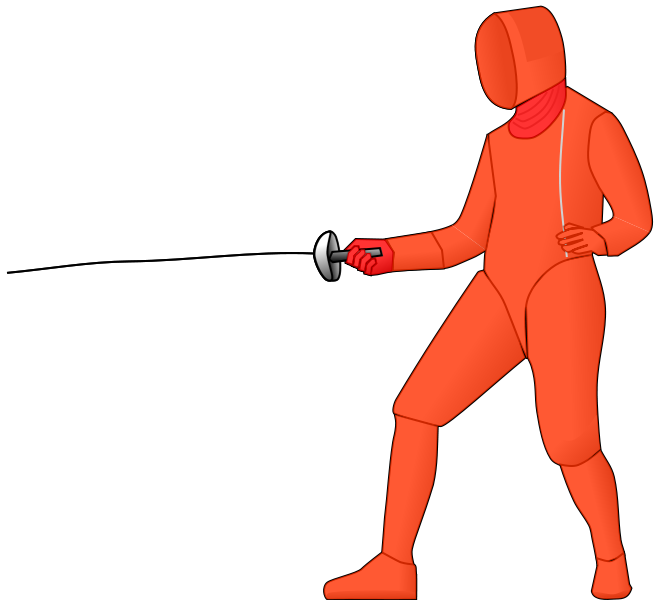
\includegraphics[width=0.4\linewidth]{blancoValido}
	\caption[Blanco válido espada]{Blanco válido espada}
	\label{fig:blancoValido}
\end{figure}


Como hemos mencionado antes es un arma de estoque, por lo que el mecanismo de activación estará en la punta
 y será mediante un botón, el cuál al presionarse sobre un blanco válido (cualquier objeto que no esté aislado en el circuito)
 cerrará un circuito eléctrico cuyo objetivo es señalizar el tocado. A partir de este
 momento el rival tiene un breve periodo de tiempo, 0.4 segundos,
 para realizar un tocado sobre el rival y que haya un tocado doble. Pasado este tiempo el circuito se bloqueará
 y solo será efectivo el primer tocado. A pesar de que haya un tocado doble no quiere decir que siempre sean válidos
 ambos tocados. Mediante las normas se dictaminará si los dos, solo uno o ninguno de ellos lo es.
 Un ejemplo podría ser que uno de los dos tiradores se encuentre fuera de la pista, lo cual anularía su tocado.
 Como se han podido dar cuenta, hemos hablado de tiempo, por lo que otro componente a tener en cuenta es ser mas
 rápido que el rival, esto habrá que tenerlo en cuenta en nuestro esquema táctico para poder decidir una acción en
 la cual, aunque nos toquen, nosotros lo hagamos con suficiente antelación al rival de modo que su tocado no
 sea válido.

% https://es.m.wikipedia.org/wiki/Archivo:Fencing_epee_valid_surfaces.svg
\begin{figure}[htb]
	\centering
	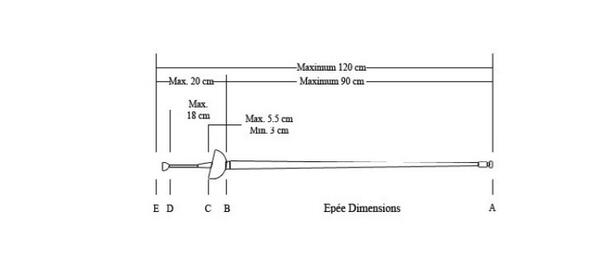
\includegraphics[width=0.9\linewidth]{epee-length-diagram}
	\caption[Dimensiones espada]{Dimensiones espada}
	\label{epee-length-diagram}
\end{figure}

Tal y como se habló antes los asaltos tienen un límite de tiempo y un límite de tocados,
 este será otro factor a tener en cuenta en nuestro esquema táctico sobre como plantear el asalto.
 Puede que a veces nos interese llevar un asalto hasta el final del tiempo desgastando físicamente al
 rival para aprovechar esta superioridad al final. Otras veces quizás nos interese lo contrario,
 acabar con el asalto cuanto antes para evitar dejar al contrario pensar. Puede que otras veces nos
 interese alargar el asalto al mayor número de tocados posibles puesto que tengamos mayor
 repertorio que nuestro oponente, mientras que en el caso contrario, si tenemos pocas acciones nos interesará
 hacer el menor número de tocados. También habrá que tener en cuenta el marcador y cuanta ventana hay
 hasta el final del combate, si al rival le falta un tocado para ganar, mientras que a nosotros nos faltan
 tres, no nos interesa que haya un tocado doble puesto que el ganaría. Estas son algunas de las variables
 que entran dentro de la formula para plantear nuestra táctica en un asalto de esgrima.

\subsection{Estructura competición esgrima}

Una vez que ya sabemos como funciona un asalto de esgrima podemos hablar sobre como funciona una competición
 de esgrima. Se explicará el funcionamiento
 de una competición estándar, el cual puede variar en función de la categoría y tipo de competición, puesto que
 existen varios formatos, como por ejemplo equipos, veteranos, competiciones amistosas, etc.
 En cuanto a las competiciones individuales primero se disputa una fase de grupos, la cual se denomina
 \textit{poule} en la cual se dividen a todos los tiradores en poules (grupos) de seis o siete tiradores en función
 del número de participantes que haya. Siendo siete el número ideal y dejando las de seis en caso de que
 no haya número suficiente de tiradores. Estas poules se hacen en función del ranking de los tiradores inscritos
 a la competición, de manera que estén lo mas equilibradas posibles. A destacar que hay un sistema para realizarlas y no
 es a intuición del directorio. Una vez organizadas las poules se da
 comienzo a ellas. En ellas se enfrentan todos los tiradores entre ellos, empezando los que sean del mismo
 país y/o club, para evitar favoritismos mas adelante. Estos enfrentamientos serán en un único asalto con un
 límite de cinco tocados y una duración máxima de tres minutos. El primero que llegue al límite con diferencia
 de un tocado o quien tenga mayor puntuación al acabar el tiempo será el ganador de este encuentro. El orden
 de enfrentamiento entre tiradores también está pre-establecido según la posición dentro de la poule.
 En el cuadro 3.1 se podrá encontrar una ejemplo de hoja de poule.

\begin{table}[htb]%
  \centering
  \caption{Ejemplo tabla resultados poule}
  \label{tab:anchura}
  \begin{tabular}{ | l | l | l | l | l | l | l | l | }
    \hline
    & Tirador 1 & Tirador 2 & Tirador 3 & Tirador 4 & Tirador 5 & Tirador 6 & Tirador 7 \\ \hline
    Tirador 1 & x & V & & & & & \\ \hline
    Tirador 2 & 1 & x & & & & & \\ \hline
    Tirador 3 & & & x & & & & \\ \hline
    Tirador 4 & & & & x & & & 2 \\ \hline
    Tirador 5 & & & & & x & & \\ \hline
    Tirador 6 & & & & & & x & \\ \hline
    Tirador 7 & & & & $V_3$ & & & x \\
    \hline
  \end{tabular}
\end{table}

La anterior tabla sería un ejemplo de una poule en mitad de una competición. Se puede apreciar como se anotan
 las victorias, las derrotas y los resultados de ambas. En caso de obtener una victoria se anotará la puntuación. Una vez
 terminadas todas las poules se obtendrá la clasificación general, obteniéndose de la siguiente manera:

\begin{enumerate}
  \item Número victorias
  \item Porcentaje Victorias/Derrotas
  \item Tocados dados - Tocados recibidos
  \item Tocados dados
\end{enumerate}

En caso de empate de todo lo anterior ambos mantendrán el mismo número de serie y se saltará el siguiente. El orden de
 quien estará encima de otro será aleatorio. Una vez obtenida la clasificación general de las poules, se hace un corte
 para eliminar a un porcentaje de los participantes, suele ser un veinte por ciento. Con los tiradores restantes
 de este corte se hace un tablón lo suficientemente grande para acoger a todos los participantes. El número de este
 tablón será una potencia de dos, es decir 2, 4, 8, 16, 32, 64, etc. En caso de no haber participantes suficientes para completar
 el tablón los primeros participantes pasarán exentos de la primera ronda. El resto de la competición es una eliminatoria
 directa en la que el vencedor pasa a la siguiente ronda mientras que el perdedor termina la competición.

Debido a que cada punto cuenta desde el inicio, ya que esto determinará como de fácil será el camino en la competición
todas y cada una de las decisiones que tomemos deberán ser lo mas óptimas posibles. Para ello muchas veces contamos
con nuestra experiencia, entrenadores o incluso compañeros que nos ayudarán a tomar una decisión dándonos su opinión.
Pero como no siempre será este el caso, se quiere desarrollar una herramienta la cual nos facilite la toma de
decisiones en mitad de la competición. Para ello usaremos un sistema de apoyo a la decisión, a partir de ahora
lo denominaremos como DSS (del inglés Decision Support System).

\newline

\section{Sistema de apoyo a la toma de decisión usando técnicas de aprendizaje automático en esgrima}
\subsection{Sistema de apoyo a la toma de decisión (DSS)}

Siempre se ha querido tomar una buena decisión y no siempre se ha podido, en la mayoría de los casos
 por no tener los conocimientos suficientes. Pero ¿qué es la mejor, una buena y una mala decisión?
 Esto es algo que, dependiendo del contexto, podría ser tanto subjetivo como objetivo. Por ejemplo, si nuestro
 objetivo es conseguir correr una maratón, no entrenar para ello posiblemente sea una mala decisión.
 Sin embargo, si hemos decidido seguir un plan de entrenamiento, el cual nos preparará para terminar
 nuestro objetivo habremos tomado una buena decisión. Pero esto sigue sin habernos contestado la pregunta
 de cuál será la mejor decisión. Bien, en este caso tendremos que entrar mas en detalle para saber
 cual es nuestro objetivo específico, en el caso de que solo sea terminarla, la mejor decisión será seguir aquel
 plan de entrenamiento que con el menor esfuerzo nos permita terminarla. Sin embargo, si nuestro objetivo
 es el de conseguir una buena marca, esta no habrá sido la mejor decisión puesto que tendremos que
 seguir un plan el cual nos permita ir mas rápido, aunque el esfuerzo sea mayor.

Una vez aclarada que es una mala, buena y la mejor decisión podremos hablar sobre lo que es un sistema
 de apoyo a la toma de decisiones. Estos son sistemas desarrollados para dar una decisión, en su mayoría
 aplicaciones informáticas, los cuales siguen el proceso de una toma de decisiones. Estos utilizan
 los datos y modelos para generar las alternativas posibles y acabar tomando la mejor decisión. Detrás
 de estos sistemas suele haber un sistema experto detrás, el cuál es un conjunto de reglas obtenidas
 a través de conocimiento extraído previamente. Dicho conocimiento se puede apoyar de otros sistemas como
 arboles de decisión o redes bayesianas para obtener conocimiento.

Un ejemplo de lo mencionado anteriormente fue en el DSS basado en redes bayesianas con una aplicación
 a la lucha contra las infecciones nosocomiales (Hela Ltifi, et al). En este caso lo que se pretendía
 era reducir el número de pacientes infectados. Para ello desarrollaron un sistema para ayudar a los
 médicos a prevenir dichas infecciones. Dicho sistema fue desarrollado mediante un proceso KDD el
 cuál se nutre de una base de datos cedida por un hospital. Dicho proceso consistía en analizar los datos
 e intentar obtener conocimiento de ellos. Para ello habría que seguir una serie de pasos como la
 limpieza, pre-procesamiento de datos, detección de patrones y ahí es cuando se podría obtener conocimiento.
 Dicho sistema ayudaría a reducir costes en los hospitales además de reducir el número de casos de infección.

\subsection{Sistemas basados en el conocimiento}

Parte de un DSS pueden ser los sistemas basados en conocimientos, los cuales parten de un conocimiento extraído de un
 experto y es transportado a una aplicación informática la cual será lo mas fiel a reproducir
 la decisión de dicho experto. Para ello se siguen una serie de procesos para poder transformar
 dicho conocimiento hacia la aplicación. Esta suele contar con una interfaz de usuario para que
 sea lo mas cómoda posible. El proceso no es trivial puesto que se necesita mínimo
 de un ingeniero de conocimiento y de un experto en la materia. Además ambos deben estar predispuestos
 a llevar a cabo el proyecto, puesto que es de vital importancia que se colabore en la mayor
 medida posible. Para ello se deberá extraer el conocimiento del experto mediante diversos métodos
 como puede ser un sistema de entrevistas, en las cuales el ingeniero le plantea una serie
 de problemas y/o dudas al experto y este deberá responderle. Una vez finalizada el ingeniero
 analizará el resultado de la entrevista, pasando a reglas dicho conocimiento o elaborando
 una nueva entrevista en caso de que fuera necesario.

Un ejemplo de lo mencionado anteriormente sería el sistema desarrollado en la universidad de Split.
 Aquí desarrollaron un sistema experto el cual era capaz de detectar talento en jóvenes que
 practicaban diferentes deportes con sus modalidades. En este caso iban un paso mas allá puesto
 que no solo jugaban con el conocimiento extraído del experto, si no que generaban una serie de
 pesos para sus reglas en conjunto de una solución ya hecha en los deportes. Esto llevó a lograr
 una aplicación en tiempo real mediante una página web en la cual cualquiera podría realizar consultas
 acerca de si una persona podría ser talentosa. A pesar de todos los esfuerzos en el propio artículo
 mencionan que no hay una respuesta definitiva y completa a la pregunta.

Por tanto nos encontramos ante la siguiente pregunta ¿Cómo nos podríamos aprovechar los
 sistemas basados en conocimiento, sistemas de apoyo a la decisión y todo lo mencionado
 anteriormente en un campeonato de esgrima? Bien pues la respuesta es desarrollar un sistema de apoyo
 a la toma de decisión, ayudado de un sistema basado en el conocimiento. Esto nos permitirá tener una
 visión mas en el campo de batalla, donde
 nuestras capacidades para tomar decisiones están limitadas, ya sea por cansancio físico, presión del
 momento, etc. Esto no sustituirá a un entrenador, puesto que hay cosas subjetivas y que requieren
 de un mayor contexto que se le pueda dar al sistema, además de la \textit{intuición} que se tiene en esos momentos
 pero si nos servirá para tener una visión más de lo que se puede hacer, que en la mayoría de los
 casos nos hará falta. A pesar de todo esto recordamos que no tomará la decisión por nosotros,
 sino que nos aconsejará y será el usuario final el que deba tomar la decisión.

\subsection{Machine Learning}
Machine Learning (ML) es una disciplina científica que se encuentra dentro de la Inteligencia
 Artificial en la cual se crean sistemas que aprenden automáticamente. Entendemos por aprender
 como la detección de patrones complejos en gran cantidad de datos. En este caso, quien aprenderá
 será un algoritmo que revisará los datos y será capaz de predecir comportamientos en un futuro.

Dentro del Machine Learning tenemos dos tipos de aprendizajes:

\begin{itemize}
  \item \textbf{Aprendizaje supervisado:} En este tipo tendremos una serie de datos de entrenamiento
    los cuales habrán sido etiquetados previamente. Con este tipo de aprendizaje tendremos clasificadores
    automáticos sin tener que programarlos. Podremos elegir la forma que tendrán.
  \item \textbf{Aprendizaje no supervisado:} Este tipo de aprendizaje es el recurrido cuando
    los datos que tenemos no están etiquetados para el entrenamiento. Es por esta razón por la que
    se procura encontrar algún patrón que simplifique el análisis.
\end{itemize}

Usaremos diferentes técnicas de ML para obtener conocimiento de una base de datos, de este modo
podremos reforzar nuestro sistema basado en el conocimiento, haciendo de este un sistema mucho mas
completo.


\chapter{Propuesta}
\label{cap:Propuesta}


\chapter{Introducción y objetivos}
\label{cap: Introducción y objetivos}

%En progreso

\section{Resumen}
Pendiente de escribir

\section{Objetivos}

El principal objetivo de este TFG es contribuir al mundo del deporte, en concreto al
 deporte de la esgrima. En comienzo de este deporte hay una gran curva de aprendizaje
 en cuanto al esquema táctico se refiere puesto que al ser un deporte minoritario los
 recursos que se le dedican son menores por lo que dificulta la expansión de conocimiento
 y por ende, la adquisición de este mismo tanto a personas que ya lo practican como aquellas
 que acaban de empezar. Se quiere reducir la inclinación de dicha curva de aprendizaje
 en el momento que tienes que aprender por ti mismo y necesitas ayuda de los demás
 para saber que acciones son las correctas y porque están mal tomadas algunas decisiones,
 al menos, hasta que te puedes valer por ti mismo como tirador que es capaz de identificar
 las acciones que están ocurriendo y analizar cuales son las mejores decisiones para contrarrestarlas.

Para ello se pretende desarrollar una aplicación la cual sea capaz de llevar a
 cabo una toma de decisiones con una serie de entradas, las cuales serán aquellas
 relacionadas con el entorno de un asalto de esgrima, como son las características
 de los tiradores, como se está desarrollando el asalto, etc.

Esta aplicación será desarrollada llevando a cabo una labor de Ingeniería de Conocimiento
 junto con una extración y análisis de datos para describir el problema, extraer
 el conocimiento de expertos, conceptualizar, formalizar e implementar dicho conocimiento
 de manera entendible para los usuarios de dicha aplicación. Dicha aplicación será un SBC
 el cual aglutine todo el conocimiento de los expertos en su conjunto, además del análisis
 de datos. Dicho sistema tendrá el objetivo darle una respuesta a un tirador de tal forma
 que este tenga un punto de vista mas para tomar sus decisiones, de tal modo que le sea mas
 fácil alcanzar la victoria. Además de ayudarle a anteponerse a su rival, también servirá
 como entrenamiento y salir de dudas cuando se quiera mejorar y adquirir conocimiento.

Esto nos lleva a la conclusión de que para alcanzar el objetivo de este TFG tendremos
 que diseñar un sistema de apoyo a la toma de decisión, con acceso mediante una aplicación
 web para darle accesibilidad al programa desde cualquier sitio.

El alcance de este proyecto está basado en los recursos disponibles para realizarlo, tanto personas como tiempo.
 Varios autores han escrito libros para plasmar su conocimiento sobre este deporte,
 ya sea como plantear la gestión de un club, como preparar a los tiradores para competiciones,
 como iniciarlos, etc. Este último caso es el de Elain Cheris hablando sobre los fundamentos
 básicos de la esgrima en las modalidades de florete y espada ya que ambas comparten
 las bases. Este libro Manual de esgrima consta de 160 páginas en el que se habla sobre
 el primer año de aprendizaje de una persona que se inicia en el deporte. Para adquirir
 este conocimiento se requiere de muchas horas de trabajo y entrevistas con profesionales
 por lo que automáticamente descartamos la modalidad de sable, ya que hay poco conocimiento
 reutilizable.

Debido a los motivos expuestos anteriormente la modalidad de sable se dejará para un futuro
 a modo de ampliación. Respecto a la modalidad de florete es cierto que comparten
 las bases pero las técnicas específicas y el conocimiento es totalmente distinto,
 ya que las propias reglas difieren entre ambas modalidades en algunos aspectos,
 por lo que se podrían utilizar partes del desarrollo pero toda la adquisición de
 conocimiento, desarrollo del sistema experto habría que realizarlo partiendo de cero.
 Para ambas modalidades hay que sumar que conseguir expertos resulta de gran dificultad
 actualmente, cosa que en un futuro lejano, tres años, espero solventar. Todo esto ha
 llevado a los objetivos expuestos anteriormente.

\section{Estructura del trabajo}

Pendiente de escribir

\section{iteraciones}


fdasfdasdfas


\section{Sistema experto}
En este apartado se tratarán los pasos que se tienen que seguir para desarrollar un sistema experto.
 En la fitura 3.1 se puede ver cual es el ciclo de vida para la creación y mantenimiento de un software
 como el mencionado anteriormente.
%En este apartado se abordarán los pasos a seguir para desarrollar un sistema experto.
 %En la figura 3.1 se puede observar el ciclo de vida de creación y mantenimiento de un software
 %de este tipo:

\begin{figure}[htb]
  \centering
    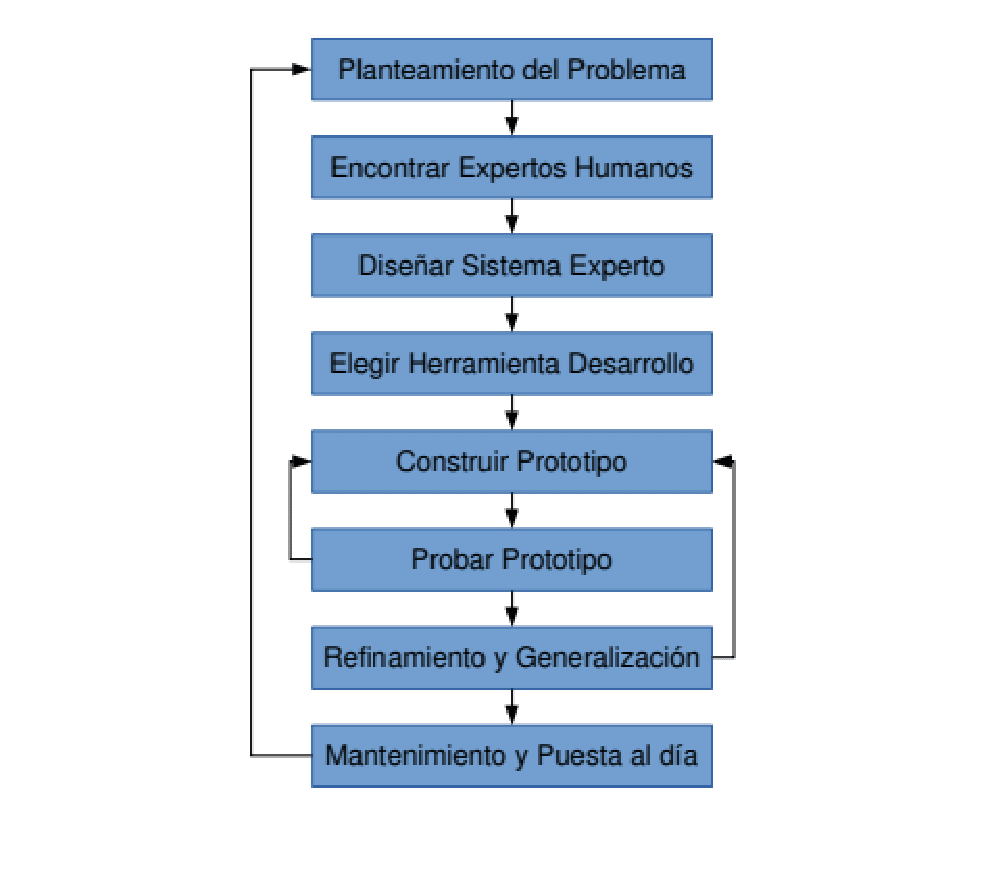
\includegraphics[width=0.4\linewidth]{DesarrolloSE}
  \caption[Desarrollo SE]{Desarrollo SE}
  \label{fig:Desarrollo Sistema Experto}
\end{figure}

A continuación se enumeran los pasos específicos para la creación del sistema experto.
\begin{enumerate}
  \item Características del sistema experto
  \item Estudio de viabilidad
  \item Adquisición del conocimiento
  \item Implantación
  \item Evaluación y pruebas
\end{enumerate}

\subsection{Características del sistema experto}
%inicio pendiente de revision palabras

Ante la situación de querer desarrollar un sistema experto lo primero que se tendrá
 que hacer será definir el alcance y los límites de dicho sistema. Esto quiere decir que
 habrá que indicar que cubre y que no nuestro sistema experto. De esta forma sabremos
 cuales son sus limitaciones y en un futuro que se podrá ampliar.

%Cuando se desea implementar un sistema experto en primer lugar se debe definir el
 %alcance y los límites de dicho sistema, se deben indicar que aspectos cubre el
 %sistema experto y que aspectos quedan fuera del ámbito del sistema.

Aquí se definirán las características del problema al que nos enfrentamos.
 La intención de este apartado es conocer cuál es la naturaleza del problema
 y que objetivos se pretenden cumplir de manera que se sepa como va a ayudar
 nuestro sistema experto a la solución de dichos problemas. Para ello habrá
 una interacción entre el ingeniero de conocimiento y el experto. El experto
 será quien enseñe al ingeniero una serie de casos y será este último el que se
 encargue de desarrollar un primer enfoque del problema. Dentro de estas interacciones
 serán las mas comunes que el ingeniero le muestre el conocimiento adquirido
 y el experto le ayude a refinar y aclarar los posibles errores. De esta manera
 y con las iteracciones que sean necesarias se acabará llegando a una descripción
 lo mas real posible.

%Define las características del problema. Se pretende determinar la naturaleza
 %del problema y los objetivos precisos que indique exactamente cómo se espera
 %que el sistema experto contribuya a la solución de los problemas. Existirá
 %una interacción entre experto e ingeniero. Cuando el experto en el dominio
 %muestre distintos casos, el ingeniero del conocimiento desarrolla una primera descripción
 %del problema. Normalmente el experto no esta de acuerdo con ella, o mejor dicho,
 %no siente que representa el problema en su totalidad, entonces el ingeniero reformulará
 %la descripción. Esta actividad prosigue hasta que los dos estén de acuerdo en la
 %descripción.

%fin pendiente de revision palabras

\subsection{Estudio de viabilidad}
%inicio pendiente de revision palabras

Una vez que se ha definido el alcance del sistema experto deberá hacerse un estudio
 previo a la implementación para conocer la viabilidad de este sistema desde un punto
 de vista computacional. Para ello se hará un estudio de viabilidad. En este caso se
 utilizará el test de SLAGEL. Este estudio establecerá si el proyecto cumple con las
 estas características:

%Teniendo claro el alcance del sistema experto debe estudiarse si la implementación
 %del mismo es posible desde el punto de vista de la computación. Para esto se
 %realiza un estudio de viabilidad, en este caso se utiliza un estudio de viabilidad basado
 %en el test de SLAGEL. Este estudio establece sie l proyecto cumple con las siguientes
 %características.

\begin{compactitem}
  \item \textbf{Plausible}: Determina si es posible resolver el problema desde el
     punto de vista de la ingeniería del conocimiento.
  \item \textbf{Justificable}: Analiza si está justificado el desarrollo del
     sistema desde la perspectiva de la ingeniería dle conocimiento, se basa en
     temas como la necesidad del sistema y la inversión a realizar.
  \item \textbf{Adecuado}: Establece si el problema a resolver está dentro
     del marco de la ingeniería del conocimiento, existen problemas que son más
     adecuados resolverlos por métodos tradicionales.
  \item \textbf{Éxito}: Determina las probabilidades de éxito del sistema a
     desarrollar, es una estimación
\end{compactitem}

El método del test de SLAGEL se define en el Anexo A.
%fin pendiente de revision palabras


\subsection{Adquisición del conocimiento}
%inicio pendiente de revision palabras


Uno de los pilares y por lo general con mayor complejidad a la hora de implementar
 un sistema experto es obtener el conocimiento, el cual suele ser a través de un experto,
 para después volcarlo en el sistema experto. Para ello hay muchos métodos y herramientas
 entre las cuales se encuentran la entrevista, observación y creación de escenarios.

%Una de las partes más importantes y a la vez más complicadas de la implementación
 %de un sistema experto es obtener el conocimiento, normalmente un experto, y
 %volcarlo en el sistema experto. Existen muchas herramientas y métodos para obtener
 %este conocimiento entre las cuales está la entrevista, la observación y la creación
 %de escenarios.

La adquisición del conocimiento trata de que las personas que no son expertas en la materia
 donde se va a implementar el sistema experto, obtengan el conocimiento necesario para ser
 capaces de resolver problemas de diferentes fuentes. El proceso de obtención del conocimiento
 sigue varias etapas las cuales se resumen en las siguientes:
%La adquisición del conocimiento es la principal complicación en el desarrollo de
 %Sistemas Expertos. Consiste en que las personas no expertas en el dominio donde
 %se va a desarrollar el Sistema Experto extraigan el conocimiento necesario para resolver
 %problemas de diversas fuentes. El proceso de adquisición del conocimiento ha seguido
 %diferentes etapas que podrían resumirse en las siguientes:

\begin{compactitem}
  \item Primeras reuniones con los expertos y evaluación de la viabilidad del proyecto.
  \item Extración de conocimientos, a partir de la documentación disponible, como
     por ejemplo libros, conferencias, internet, etc.
  \item Deducción de conocimientos a partir de los expertos.
\end{compactitem}

Además se logra la familiarización del Ingeniero del Conocimiento en el contexto en
 el que se va a trabajar. Se busca en las primeras reuniones describir conocimientos
 generales, así como afianzarse con la terminología.

La estructura de las entrevistas junto a casos de entrevistas se define en el anexo B.

Después de obtener el conocimiento será definir unas estructuras para poder organizarlo.
 Será en esta etapa donde el ingeniero del conocimiento decide que estructuras serán
 las mas adecuadas para este sistema experto, eso si, previamente tiene que estar perfectamente
 definido el problema en toda su magnitud, sin haber hecho referencia a técnicas de programación
 o solo habiendo tenido en cuenta métodos exitosos en IA. Con estructura adecuada se hace referencia
 aquella que da una solución total o parcial al problema analizado previamente. Una de las
 diferentes responsabilidades del ingeniero de conocimiento será analizar situaciones tipo y
 a partir de ellas extraer las reglas que serán las que describan el conocimiento del experto
 en la materia.

%Una vez obtenido el conocimiento hay que designar estructuras para organizar el
 %el conocimiento. Después de haber determinado el problema en toda su magnitud,
 %sin haberse referido a técnicas de programación o a indagar solo en los métodos
 %que son exitosos en inteligencia artificial, es en esta etapa donde el ingeniero del
 %conocimiento selecciona las estructuras apropiadas a este sistema experto en particular.
 %Es decir, que dan solución total o parcial al problema analizado en las etapas precedentes.
 %Una de las responsabilidades principales del ingeniero del conocimiento es analizar
 %situaciones tipo y a partir de ellas extraer las reglas que describen el conocimiento del
 %experto en el dominio.

%fin pendiente de revision palabras

\subsection{Implantación}
%inicio pendiente de revision palabras

Desarrolla la transformación de los conocimientos representados en el modelo formal
 en un modelo computable.

Será en esta etapa en la que se elaboren las reglas que lleven el conocimiento adquirido
 previamente. Se utilizarán las herramientas y técnicas predeterminadas para implementar
 un prototipo del sistema. Este prototipo será utilizado para probar y evaluar los avances
 que se hacen en el proyecto. Se volverá a etapas anteriores en caso de que el resultado
 no sea satisfacotrio para poder perfeccionarlo. Cuando haya alcanzado un grado optimo
 de satisfacción como para poder ser ejecutado, el sistema experto estará listo para ser probado.

%Elaboración de las reglas que incorporen el conocimiento. Se peretende en esta ocasión
 %usar las herramientas y técnicas predeterminadas para implementar una primera versión
 %o prototipo del sistema. Este prototipo esta destinado a evaluar los progresos que se
 %van haciendo, y por ende, retornar a etapas anteriores si es necesario.

%Una vez que el sistema prototipo se ha perfeccionado lo suficiente para ser ejecutado,
 %el sistema experto estará listo para ser probado.

%fin pendiente de revision palabras

\subsection{Evaluación y pruebas}
%inicio pendiente de revision palabras

En esta fase se establece el grado de experiencia que adquirió el sistema. Cualquier
 experto en la materia, hayan o no participado en el proyecto, se comprometen a evaluar
 la capacidad del sistema. Estos expertos trataran de entrever la calidad de dicho sistema
 asistiendo en diferentes casos de problemas que tendrá que resolver el software. Otra de
 las cosas que tendránque evaluar será la amplitud que posee el repositorio de casos y como
 el sistema experto guía su uso.

%Establece el grado de experiencia alcanzado por el sistema. De manera tal que expertos
 %en el área que han o no partilcipado en el desarrollo del proyecto se comprometen a
 %evaluar el desempeño del sistema, tratando de vislumbrar la calidad de asistencia que
 %brinda el Sistema Experto ante diferentes casos de problemas a resolver por software.
 %También se evalúa la amplitud y generalidad de marcos compuestos que posee el repositorio
 %y cómo el sistema guía su uso.

Una vez el sistema sea capaz de llevar a cabo el mismo trabajo que haría un especialista
 podremos decir que está preparado.


%Se considera que el sistema experto está terminado cuando realiza trabajos a nivel
 %del especialista. Entonces, el proceso de prueba no esta listo hasta que las soluciones
 %propuestas por el sistema seantan válidas como las propuestas por el experto humano.
%fin pendiente de revision palabras

\subsection{Motor de inferencia}
%inicio pendiente de revision palabras
El sistema experto que se va a desarrollar siguiendo la metodología anterior va
 a funcionar sobre un motor de inferencia desarrollado para tal fin, el motor
 de inferencia se basa en el motor implementado para CLIPS y a continuación se van
 a detallar las características de dicho motor.

\subsubsection{Algoritmo de selección de reglas aplicables en CLIPS}
\begin{compactitem}
  \item Elegir la regla aplicable con máxima prioridad.
  \item Elegir la regla según estrategia de resolución de conflictos.
  \item Elegir de forma arbitraria.
\end{compactitem}

Estas son las estrategias definidas en el motor de inferencia de CLIPS para
 la selección de reglas aplicables o activas son varias:

\begin{compactitem}
  \item \textbf{Depth Strategy (estrategia por defecto)}. Una activación que contiene el hecho
    más reciente se sitúa por encima de las activaciones con igual o mayor antigüedad.
 \item \textbf{Breadth Strategy}. Una activación que contiene el hecho más reciente se
    sitúa por debajo de las activaciones con igual o mayor antigüedad.
 \item \textbf{Complexity Strategy}. Las nuevas activaciones se sitúan por encima de las
    activaciones con igual o menor especificidad (no de comparaciones que han de
    realizarse en el antecedente una la regla).
 \item \textbf{Simplicity Strategy}. Las nuevas activaciones se sitúan por debajo de las
    activaciones con igual o mayor especificidad.
 \item \textbf{LEX Strategy}. Se ordenan los time-tag en orden decreciente y se comparan
    uno a uno, hasta encontrar uno mayor que otro, en caso de que no haya el mismo
    número de time-tag se añaden ceros al final.
 \item \textbf{MEA Strategy}. Parecido a LEX, pero mirando sólo el primer patrón que
    equipara en la regla.
 \item \textbf{Random Strategy}. A cada activación se le asigna un número aleatorio para
    determinar su orden en la agenda.
\end{compactitem}

\subsubsection{Definición de prioridades en CLIPS}
\begin{compactitem}
  \item Asignar un valor de prioridad (entero positivo) a cada regla.
  \item En CLIPS se definen como propiedades de reglas.
  \item Se recomienda minimizar el uso de prioridades de reglas.
\end{compactitem}

%fin pendiente de revision palabras

%\section{Herramienta web}

En este apartado se tratarán los pasos a seguir para desarrollar la herramienta web
 que de visibilidad, acceso y uso al sistema experto.

\subsection{Metodología SCRUM}

Para el desarrollo e implementación de la herramienta web se usó una metodología basada en SCRUM.
 Tendremos un modelo de desarrollo el cual será iterativo e incremental. Dicho modelo tiene
 las siguientes características:

\subsubsection{Iteraciones}

Una iteración también es conocida como "sprint". Estamos hablando de iteraciones dentro del
 proceso de desarrollo cuya duración será de entre 7 y 30 días, dependiendo del número de
 objetivos que se quieran cumplir y la demanda de la planificación. Al finalizar el srpint
 se obtendrá un incremento del producto, lo cual será un resultado válido y con suficiente
 calidad como para poder ser utilizado.

\begin{figure}[htb]
  \centering
    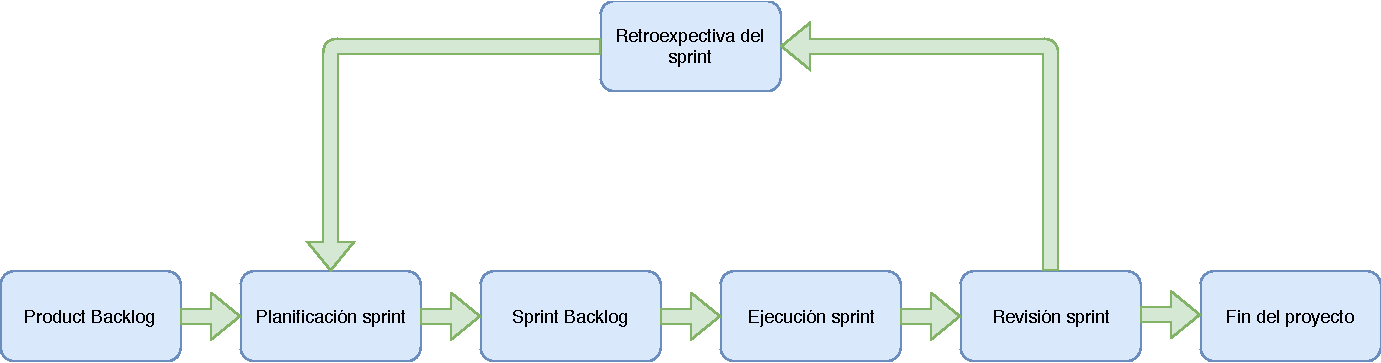
\includegraphics[width=0.4\linewidth]{Scrum}
  \caption[Desarrollo herramienta web]{Desarrollo herramienta web}
  \label{fig:Desarrollo herramienta web}
\end{figure}

Para este proyecto se han utilizado sprints de 30 días para asegurar el cumplimiento de estos.
 La distribución del tiempo fue de 75\% para realizar tareas del sprint en manera de cola de
 prioridad. Dentro de estas tareas se incluye el desarrollo de las pruebas necesarias y la
 comprobación de funcionalidades de las mismas. El resto 25\% se utilizó para el estudio del
 actual sprint para mejora de los siguientes, planificación y organización del siguiente sprint.
 En el capítulo de evaluación encontraremos la tabla con los sprints realizados y la funcionalidad
 desarrollada dentro de este.

\subsubsection{Definición de elementos}

Para la comprensión y buen desarrollo de esta metodología hace falta definir una serie
 de elementos los cuales son los siguientes:

\begin{itemize}
  \item \textbf{Product Backlog:} Será una lista de todos los requisitos del sistema, también
     conocido como historias de usuario. Estos requisitos estarán descritos en alto nivel
     de modo que cualquiera pueda entenderlo y estos estarán priorizados. Esta lista
     podrá verse modificada una vez iniciado el proyecto y en cualquier momento del ciclo de vida.
  \item \textbf{Sprint Backlog:} Esta será la lista de tareas a desarrollar durante el sprint
     para poder llegar al incremento planificado. Cada tarea deberá tener un tiempo estimado
     y los recursos que se necesitan para llevarlas a cabo. Cada tarea no deberá tener una
     estimación mayor de 24 horas puesto que esto indicaría que es demasiado larga y podría
     complicar el cumplimiento del resto de tareas para la fecha acordada. En caso de que
     alguna tarea supere dicho tiempo deberá ser dividida en subtareas.
  \item \textbf{Incremento:} Será el resultado esperado y obtenido al finalizar el sprint. Dicho
     resultado deberá ser terminado y poder ser utilizado.
\end{itemize}

En el caso de este proyecto, el producto backlog estará compuesto desde el principio de todas
 las funcionalidades que se desean implementar. Estas fueron obtenidas a raíz de la metodología
 de desarrollo. Para obtener mayor información sobre dichas funcionalidades deberemos consultar
 el siguiente capítulo en el cual se hablan de las mismas en profundidad.

Estas funcionalidades no serán las únicas en el product backlog puesto que durante el desarrollo
 e implementación del proyecto pueden surgir nuevas que no se hayan identificado en la etapa
 de captura de requisitios. Este caso ocurrio con el desarrollo del manual de usuario,
 informes para mostrar los resultados obtenidos y pequeñas mejoras identificadas al entregar
 el producto al final de cada sprint.

\subsubsection{Definición de roles}

Dentro de un equipo que trabaje en esta metodología habrá dos grupos de personas. El primer grupo
 de personas tendrán los siguientes roles:

\begin{itemize}
  \item \textbf{Product Owner:} Será el encargado de dar voz al cliente. En el caerá la
     responsabilidad de escribir las historias de usuario y ordenarlas en el product backlog.
   \item \textbf{Scrum Master:} Será el encargado de asegurarse que todo va bien en cuanto
      al proceso de desarrollo y este se cumple. Además intentará, en la medida de lo posible,
      evitar el mayor número de incidencias posibles.
   \item \textbf{Equipo:} Serán aquellos que se encarguen de realizar el desarrollo del producto.
\end{itemize}

En este proyecto el tutor del trabajo de fin de grado será quien adopte el rol de product owner
 y scrum master, mientras que el alumno ha sido formado por el autor del proyecto.

El otro grupo no entrará direcamente como parte del proceso, pero habrá que tenerlos en
 cuenta ya que serán ellos quienes nos den información al finalizar el sprint. De esta
 información podremos mejorar nuestro producto, aunque esto conllevará cambios en los
 siguientes sprints. Los usuarios que están dentro de este grupo serán aquellos que usen
 la herramienta, el usuario final. En nuestro caso serán los entrenadores y esgrimistas
 durante las competiciones o entrenamientos.

\subsubsection{Definición de reuniones}

Dentro de scrum existen diferentes tipos de reuniones. Estas reuniones son utilizadas para
 planificar las tareas del sprint, analizar las nuevas tareas que se han de incorporar en
 el product backlog, seguir el estado de salud del sprint y también comprobar cuales fueron
 los resultados de los sprints. Las diferentes reuniones que se llevan a cabo son las siguientes:

\begin{itemize}
  \item \textbf{Planificación del sprint:} En esta reunión se eligen las tareas del product
     backlog según estén ordenadas para mantener la prioridad de estas. Estas tareas deberán
     estar estimadas y hacerlo en caso de que no lo estén. En función del tiempo y recursos
     disponibles para el sprint se deberán escoger mas o menos tareas. Una vez seleccionadas
     tendremos el sprint backlog.
  \item \textbf{Seguimiento del sprint:} Esta será una reunión diaria de muy corta duración.
     El principal objetivo de esta reunión será conocer el estado de salud del sprint, de modo
     que se puedan tomar las medidas oportunas para que todo el trabajo salga adelante. Un
     claro ejemplo sería un bloqueo entre recursos que no se ha detectado previamente. Para
     ello cada miembro del equipo deberá comentar por encima cual fue su trabajo del día
     anterior junto con lo que tiene previsto para la jornada actual. No se deberán abordar
     problemas en esta reunión si se hará fuera de esta. Esta reunión es solo para estar al
     tanto de los posibles problemas.
  \item \textbf{Revisión del sprint:} En esta reunión se revisará el trabajo realizado y cuál
     faltó por completar. Además se presentará el incremento obtenido y se analizará el motivo
     de aquellas tareas que no se terminaron.
\end{itemize}


\subsubsection{Ciclo de vida SCRUM}

El ciclo de vida de SCRUM está formado por cinco fases, dichas fases son: concepto, especulación,
 exploración, revisión y cierre. A continuación se explican con mas detalle.

\begin{itemize}
  \item \textbf{Concepto:} Esta será la primera fase del ciclo de vida. Aquí será donde se sacará
     una primera idea sobre el producto realizada por el el cliente. También se definirá el alcance
     y el equipo de trabajo.
  \item \textbf{Especulación:} Una vez definido el alcance y con una visión del producto, se lanzarán
     hipotesis sobre lo que se desea obtener. Una vez lanzadas, se tendrá que hacer un contraste
     con la realidad. Esta fase se llevará a cabo en todas y cada una de las iteraciones del desarrollo.
  \item \textbf{Exploración:} Aquí será donde se lleven a cabo los incrementos del producto mediante
     el desarrollo de las funcionalidades definidas.
  \item \textbf{Revisión:} En esta fase se comprobará que se lleva a cabo la visión del producto, además
     de los objetivos que se han marcado para él.
  \item \textbf{Cierre:} Esta será la fase final del ciclo repetitivo, en la que se entregará
     el producto listo, funcional y revisado.
\end{itemize}

\textbf{Concepto}

Aquí definimos que producto queremos conseguir y como queremos conseguirlo. En este caso
 nuestro objetivo es elaborar una herramienta que permita apoyar a la decisión de una táctica
 en un asalto de esgrima. Para ello se optará por una aplicación web en la que puedas
 introducir los datos de los tiradores y que te aconseje sobre las acciones que debes o no
 hacer. Para ello deberá cumplir con tener una interfaz amigable, fácil y rápida de usar puesto
 que se usará en momentos de inquietud.

\textbf{Especulación}

En el caso de este proyecto las hipotesis lanzadas fueron transformadas a funcionalidades
 para una mayor visibilidad y comprensión de las mismas. Estas funcionalidades se han descrito
 mediante casos de uso. Dichos casos de uso se analizaron al comiendo del proyecto. Además, al
 finalizar cada sprint, después de un análisis, se incluyeron mejoras para el proyecto.

\textbf{Exploración}

Para la implementación de las funcionalidades deseadas se ha utilizado el paradigma de orientación a objetos
 usando un patrón de programación Modelo-Vista-Controlador. Esta es una de las
 razones por la que se eligió el lenguaje Ruby, ya que
 fue diseñado específicamente para ello. Además, es el más utilizado en dicho paradigma para el
 desarrollo de aplicaciiones web de desarrollo ágil. En concreto sacaremos especial partido
 a la parte de Vista-Controlador puesto que serán los controladores los que se encarguen de
 toda la lógica de la aplicación, entre ella estará el sistema experto y las decisiones que se toman.
 Las vistas serán las que se encarguen de recoger la información y enviarla a los controladores.
 Una vez que estos han procesado los datos y tienen un veredicto, de nuevo las vistas serán
 quienes tendrán la responsabilidad de mostrar los resultados de una manera entendible y
 de visionado rápido al usuario.

\textbf{Revisión}

En esta fase se fijarán las reuiones de fin de sprint, en las cuales se verificará que se
 han alcanzado todos los objetivos puestos para el sprint. También se comprobará que el producto
 se adecua a las funcionalidades que se planificaron.

\textbf{Cierre}

Esta será la fase en la que se hizo entrega del producto. Para ello tuvo que terminarse
 la implementación y aceptación de todas las funcionalidades que se describieron al inicio
 del proyecto, establecidas en el product backlog. Tener en cuenta que también han de cumplir
 lo anterior aquellas mejoras propuestas durante el desarrollo del proyecto.

La herramienta actualmente está en estado de mantenimiento, con lo cual se seguirá mejorando
 mediante nuevas funcionalidades propuestas por los usuarios de esta misma que pueden enviar
 en la propia herramienta.


\chapter{Desarrollo}
\label{cap:Desarrollo}

\chapter{Introducción y objetivos}
\label{cap: Introducción y objetivos}

%En progreso

\section{Resumen}
Pendiente de escribir

\section{Objetivos}

El principal objetivo de este TFG es contribuir al mundo del deporte, en concreto al
 deporte de la esgrima. En comienzo de este deporte hay una gran curva de aprendizaje
 en cuanto al esquema táctico se refiere puesto que al ser un deporte minoritario los
 recursos que se le dedican son menores por lo que dificulta la expansión de conocimiento
 y por ende, la adquisición de este mismo tanto a personas que ya lo practican como aquellas
 que acaban de empezar. Se quiere reducir la inclinación de dicha curva de aprendizaje
 en el momento que tienes que aprender por ti mismo y necesitas ayuda de los demás
 para saber que acciones son las correctas y porque están mal tomadas algunas decisiones,
 al menos, hasta que te puedes valer por ti mismo como tirador que es capaz de identificar
 las acciones que están ocurriendo y analizar cuales son las mejores decisiones para contrarrestarlas.

Para ello se pretende desarrollar una aplicación la cual sea capaz de llevar a
 cabo una toma de decisiones con una serie de entradas, las cuales serán aquellas
 relacionadas con el entorno de un asalto de esgrima, como son las características
 de los tiradores, como se está desarrollando el asalto, etc.

Esta aplicación será desarrollada llevando a cabo una labor de Ingeniería de Conocimiento
 junto con una extración y análisis de datos para describir el problema, extraer
 el conocimiento de expertos, conceptualizar, formalizar e implementar dicho conocimiento
 de manera entendible para los usuarios de dicha aplicación. Dicha aplicación será un SBC
 el cual aglutine todo el conocimiento de los expertos en su conjunto, además del análisis
 de datos. Dicho sistema tendrá el objetivo darle una respuesta a un tirador de tal forma
 que este tenga un punto de vista mas para tomar sus decisiones, de tal modo que le sea mas
 fácil alcanzar la victoria. Además de ayudarle a anteponerse a su rival, también servirá
 como entrenamiento y salir de dudas cuando se quiera mejorar y adquirir conocimiento.

Esto nos lleva a la conclusión de que para alcanzar el objetivo de este TFG tendremos
 que diseñar un sistema de apoyo a la toma de decisión, con acceso mediante una aplicación
 web para darle accesibilidad al programa desde cualquier sitio.

El alcance de este proyecto está basado en los recursos disponibles para realizarlo, tanto personas como tiempo.
 Varios autores han escrito libros para plasmar su conocimiento sobre este deporte,
 ya sea como plantear la gestión de un club, como preparar a los tiradores para competiciones,
 como iniciarlos, etc. Este último caso es el de Elain Cheris hablando sobre los fundamentos
 básicos de la esgrima en las modalidades de florete y espada ya que ambas comparten
 las bases. Este libro Manual de esgrima consta de 160 páginas en el que se habla sobre
 el primer año de aprendizaje de una persona que se inicia en el deporte. Para adquirir
 este conocimiento se requiere de muchas horas de trabajo y entrevistas con profesionales
 por lo que automáticamente descartamos la modalidad de sable, ya que hay poco conocimiento
 reutilizable.

Debido a los motivos expuestos anteriormente la modalidad de sable se dejará para un futuro
 a modo de ampliación. Respecto a la modalidad de florete es cierto que comparten
 las bases pero las técnicas específicas y el conocimiento es totalmente distinto,
 ya que las propias reglas difieren entre ambas modalidades en algunos aspectos,
 por lo que se podrían utilizar partes del desarrollo pero toda la adquisición de
 conocimiento, desarrollo del sistema experto habría que realizarlo partiendo de cero.
 Para ambas modalidades hay que sumar que conseguir expertos resulta de gran dificultad
 actualmente, cosa que en un futuro lejano, tres años, espero solventar. Todo esto ha
 llevado a los objetivos expuestos anteriormente.

\section{Estructura del trabajo}

Pendiente de escribir

\section{Iteración 1: Obtención del conocimiento}

Una vez establecido el tema a tratar en el proyecto y el alcance del mismo,
se procede a desarrollar cada una de las iteraciones que lo componen.

En la primera iteración se ilustra el proceso de adquisicón del conocimeinto,
lo que dará una visión mas detallada del proeycto y establecerá las bases
para el desarrollo del arbol táctico que nos ayudará en la toma de decisiones en un asalto de esgrima.

\subsection{Adquisición conocimiento básico}

Lo primero que se hizo fue una investigación previa para asentar unas bases de conocimiento
básicas sobre la materia en cuestión. Para ello se hicieron diversas búsquedas por internet
buscando información acerca del deporte y su competición. Sacando bastante información
en las páginas de la federación internacional y española. Además de diversos medios como
el podcast \textit{Llamada a pista}\footnote{\url{https://llamadaapista.com/}} y redes sociales como \textit{weareeelgato}\footnote{\url{https://weareelgato.com/}}.

Sobre estas búsquedas se pudo sacar información acerca del reglamento, el cuál es algo
básico de entender para saber como se puede plantear una estrategia. También se obtuvo
información sobre los movimientos básicos de la esgrima, de este modo podríamos entender
la jerga del deporte cuando nos reunieramos con los expertos. En cuanto al contenido
multimedia se pudo sacar en claro como era un asalto de esgrima, afianzando todo el conocimiento
obtenido anteriormente, viendo los movimientos que realizaban los tiradores y como
se aplicaban las normas en los distintos casos. Además, se pudo ver como estos adaptaban
sus estilos según transcurría el combate, por lo que nos hacía ver como se planteaba
una táctica u otra en función de las características del asalto.

\subsection{Adquisición conocimiento mediante entrevistas}
%Explicar las entrevistas que se hicieron, como fueron, como se analizaron y las conclusiones
%que se hicieron sobre cada una.

Una vez que ya teníamos un conocimiento básico sobre la esgrima en la modalidad de espada,
estabamos preparados para la primera entevista con el experto. En la primera entrevista el
objetivo principal no era más que poner en claro nuestros conceptos básicos para asegurarnos
que podíamos entendernos con el experto, aunque no supieramos el razonamiento de cada caso,
pero sí el que nos decía. Es por esto por lo que se decidió una entrevista abierta semi-estructurada.

La primera entrevista se dividiría en dos partes principales. La primera de ellas sería
asegurar los conceptos adquiridos en la materia y aclarar los que no tuvieramos seguros.
Además se corregirían aquellos que fueran erroneos. La segunda parte de la entrevista
sería prácticamente abierta en su totalidad, ya que sería el experto el que nos tendría
que introducir en la materia de escoger una táctica u otra. Para ello fuimos con unas
preguntas básicas, las cuales son comunes a la mayoría de procesos de toma de decisiones.

Una vez finalizada la entrevista se analizarían los resultados y sacarían conclusiones de la misma.
El documento de la primera entrevista se puede ver en el \hyperref[cap:Entrevistas]{Anexo A}.

Con la primera entrevista finalizada y después de analizar los resultados sacamos en claro
las siguientes conclusiones:

\begin{itemize}
  \item Lo primero en lo que hay que fijarse para planificar una estrategia es en la distancia,
    físico y experiencia.
  \item La distancia se valorará según la diferencia de altura entre tiradores y el puño usado
    de cada uno.
  \item La experiencia puede jugar a tu favor si eres el que más tiene.
  \item El físico influye a la hora de escoger como quieres llevar el asalto.
  \item La personalidad del tirador influye en su forma de tirar. Intentar averiguar como es esa persona
    antes de un asalto.
  \item No hay una preferencia ante ceder terreno o llevar al rival a final de pista. Dependerá de la
    situación del asalto.
\end{itemize}

Además sacamos las siguientes palabras para el glosario:

\begin{enumerate}

  \item Cualidades del tirador
  \item Distancia
  \item Experiencia
  \item Físico
  \item Técnicas
  \item Tocar
  \item Entrar con hierro
  \item Entrar con segunda intención
  \item Altura
  \item Puño
  \item Francés
  \item Anatómico
  \item Más joven
  \item Más rápido
  \item Sentirse intimidado
  \item Saber mucho
  \item Ganar rápido
  \item Echado hacia delante
  \item Esperar
  \item Provocar errores
  \item Contra
  \item Ser ofensivo
  \item Alcance
  \item Poco contacto en hierro
  \item Perder distancia
  \item Puntería
  \item Ser pasivo
  \item Parar bien
  \item Buen contrataque
  \item Dejar corto
  \item Dejar pensar

\end{enumerate}

También actualizamos las tablas de objeto, atributo y valor (ver \hyperref[tab:Tabla objeto atributo y valor]{tabla 5.3})

\begin{table}[]
  \centering
  \caption{Tabla objeto atributo y valor}
  \label{tab:Tabla objeto atributo y valor}
  \begin{tabular}{lll}
    Objeto & Atributo & Valor \\ \hline
    \multicolumn{1}{l|}{\multirow{4}{*}{Tirador}} & Puño & \{Francés, Anatómico\} \\ \cline{2-3}
    \multicolumn{1}{l|}{} & Altura & {[}0, 230{]} cm \\ \cline{2-3}
    \multicolumn{1}{l|}{} & Intimidado & \{Si, No\} \\ \cline{2-3}
    \multicolumn{1}{l|}{} & Edad & {[}0, 120{]} Años \\ \cline{2-3}
  \end{tabular}
\end{table}

Una vez reposado el conocimiento adquirido podremos pasar a la siguiente entrevista,
de este modo ampliaremos la batería de posibilidades.

El planteamiento de la segunda entrevista era afianzar los conocimientos adquiridos en
la primera y ampliar estos. Para ello lo primero que se hizo fue hacer preguntas abiertas
sobre ciertas acciones en concreto. De esta manera nos aseguraríamos que estamos entiendo
bien el contexto del problema. Después pasaríamos a ampliar el conocimiento, de nuevo
con preguntas abiertas para conseguir desarrollar un esquema táctico mas amplio y complejo.

\begin{itemize}
  \item El físico es importante pero no lo único a tener en cuenta. Los reflejos será
    algo muy a tener en cuenta junto a la velocidad de reacción.
  \item La teoría no lo es todo, también habrá que detectar como de bueno es el rival
    en las dos acciones principales de todo arte marcial, la defensa y el ataque.
    Con esto podremos trazar una táctica mas fiable y eficaz.
  \item La confianza en cada uno de los tiradores será determinante para saber
    que podemos movimientos podremos llevar a cabo o no.
\end{itemize}

Además sacamos las siguientes palabras para el glosario:

\begin{enumerate}
  \item Coupé
  \item Guardia
  \item Defensa
  \item Contra-ataque
  \item Finta
  \item Provocar
  \item Engañar
  \item Distraer
  \item Llamada
  \item Finta-Pase
  \item Reflejos
  \item Capacidad defensiva
  \item Capacidad ofensiva
  \item Confianza
  \item Explosividad
\end{enumerate}

También ampliamos las tablas de objeto atributo-valor. Ver \hyperref[tab:Tabla objeto atributo y valor ampliada]{tabla 5.4}

\begin{table}[]
  \centering
  \caption{Tabla objeto atributo y valor ampliada}
  \label{tab:Tabla objeto atributo y valor ampliada}
  \begin{tabular}{lll}
    Objeto & Atributo & Valor \\ \hline
    \multicolumn{1}{l|}{\multirow{4}{*}{Tirador}} & Confianza & \{Si, No\} \\ \cline{2-3}
    \multicolumn{1}{l|}{} & Reflejos & \{Bajo, Medio, Alto\} \\ \cline{2-3}
    \multicolumn{1}{l|}{} & Velocidad & \{Bajo, Medio, Alto\} \\ \cline{2-3}
    \multicolumn{1}{l|}{} & Capacidad defensiva & \{Bajo, Medio, Alto\} \\ \cline{2-3}
    \multicolumn{1}{l|}{} & Capacidad ofensiva & \{Bajo, Medio, Alto\} \\ \cline{2-3}
  \end{tabular}
\end{table}


El glosario final se puede ver en el \hyperref[cap:glosario sistema experto]{anexo B}.
La tabla de objeto, atributo y valor final se puede ver en el \hyperref[cap:Reglas del sistema experto]{anexo C}.


%\chapter{Evaluación}
\label{cap:Evaluación}

\section{Características del sistema experto}

%inicio pendiente de revision palabras
%Pendiente de escribir

%fin pendiente de revision palabras

\section{Estudio de viabilidad}
%inicio pendiente de revision palabras
Se procederá a realizar un estudio de viabilidad basado en el test de SLAGEL, este test
 asigna pesos a una serie de características a evaluar divididas en diferentes categorías,
 después de los cálculos pertinentes se obtiene un porcentaje de viabilidad, para obtener
 un porcentaje real se procederá por último a normalizar el resultado obtenido, en el apartado
 anterior puede encontrarse la definición del método seguido para el cálculo del estudio de
 viabilidad.

Para poder entender el significado de las tablas se han usado los siguientes acrónimos
 ES: Expertos TA: Tarea DU: Directivos/Usuarios E: Esencial D: Deseable

\textbf{Características de Plausibilidad}

\begin{table}[htb]%
  \centering
  \caption{Tabla con las características de plausibilidad}
  \label{tab:anchura}
  \begin{tabular}{ | l | l | l | l | p{8cm} | l | }
    \hline
    Cat. & Iden & Peso & Valor & Denominación & Tipo \\ \hline
    EX & P1 & 10 & 10 & Existen Expertos & E \\ \hline
    EX & P2 &  10 & 9 & El experto asignado es genuino & E \\ \hline
    EX & P3 & 8 & 9 & El experto es cooperativo & D \\ \hline
    EX & P4 & 7 & 8 & El experto es capaz de articular sus métodos pero no categoriza & D \\ \hline
    TA & P5 & 10 & 9 & Existen suficientes casos de prueba; normales, típicos, ejemplares, correosos, etc & E \\ \hline
    TA & P6 & 10 & 9 & La tarea está bien estructurada y se entiende & D \\ \hline
    TA & P7 & 10 & 9 & Solo requiere habilidad cognoscitiva (no pericia física) & D \\ \hline
    TA & P8 & 9 & 8 & No se precisan resultados óptimos sino sólo satisfactorios, sin comprometer el proyecto & D \\ \hline
    TA & P9 & 9 & 7 & La tarea no requiere sentido común & D \\ \hline
    DU & P10 & 7 & 9 & Los directivos están verdaderamente comprometidos con el proyecto & D \\ \hline
  \end{tabular}
\end{table}

\textbf{Fundamentos de plausibilidad}

A continuación se fundamentan algunos de los valores elegidos para las características de Plausibilidad


\begin{compactitem}
  \item[\textbf{P1}:] Actualmente se dispone de muchos expertos en el sector. Toda sala de esgrima
     tiene un maestro el cual es un experto, con mayor o menor experiencia, el cual transmite
     sus conocimientos adquiridos con los años y los sucesos que vivió a sus alumnos. Por lo tanto
     podríamos decir que hay al menos un experto por sala de esgrima.
  \item[\textbf{P3}:] El experto escogido tiene especial interés en el proyecto, puesto que
     serviría de gran ayuda para sus alumnos en competiciones dado que actualmente es el único
     en poder dar apoyo a estos en esas situaciones.
  \item[\textbf{P7}:] Unicamente se requiere el conocimiento suficiente y experiencia en competición
     para poder identificar las acciones del rival para poder decidir que acciones llevar a cabo
     de manera que se contrarresten las del rival.
  \item[\textbf{P9}:] Al ser una serie de casos con unas entradas y salidas bien definidas, no requiere
     de un gran ingenio poder llevar a cabo la decisión, una vez tengamos todos los casos, o el mayor
     número de estos posibles, identificados.
\end{compactitem}


\textbf{Características de justificación}
\begin{table}[htb]%
  \centering
  \caption{Tabla con las características de justificación}
  \label{tab:anchura}
  \begin{tabular}{ | l | l | l | l | p{8cm} | l | }
    \hline
    Cat. & Iden & Peso & Valor & Denominación & Tipo \\ \hline
    EX & J1 & 10 & 9 & El experto no esta disponible & E \\ \hline
    EX & J2 & 10 & 8 & Hay escasez de experiencia humana & D \\ \hline
    TA & J3 & 8 & 9 & Existe la necesidad de experiencia simultánea en muchos lugares & D \\ \hline
    TA & J4 & 10 & 7 & Necesidad de experiencia en entornos hostiles, penosos y/o poco gratificantes & D \\ \hline
    TA & J5 & 8 & 9 & No existen soluciones alternativas admisibles & E \\ \hline
    DU & J6 & 10 & 9 & Se espera una alta tasa de recuperación de la inversión & D \\ \hline
    DU & J7 & 10 & 9 & Resuelve una tarea útil y necesaria & E \\ \hline
   \end{tabular}
\end{table}

\textbf{Fundamentos de justificación}
A continuación se fundamentan algunos de los valores elegidos para las características de justificación

\begin{compactitem}
  \item[\textbf{J1}:] En competiciones, sobre todo regionales y clubes pequeños, el experto
     no suele estar disponible puesto que en la mayoría de las ocasiones tiene otras labores
     como directorio técnico o incluso ser el mismo un partipante mas de la competición.
     En el mejor de los casos de que no tenga ninguan de estas labores lo normal será que
     tenga a varios alumnos que atender a la vez, por lo que será una situación común que no esté libre.
  \item[\textbf{J3}:] Se puede dar el caso de que dos alumnos de un mismo maestro tengan un
     asalto en el mismo instante. Este no podrá estar en ambos sitios a la vez y tampoco es
     aconsejable estar poco tiempo en uno, después ir al otro y así sucesivamente, por lo que
     se ve la necesidad de este conocimiento en el mismo instante en distintos lugares.
  \item[\textbf{J7}:] Al resolver la tarea de las incertidumbres sobre que hacer
     en cada una de las situacione será mas accesible el deporte para aquellos que estén
     empezando, puesto que no generará esos sentimientos de frustración por no saber que hacer.
\end{compactitem}

\textbf{Características de adaptación}
\begin{table}[htb]%
  \centering
  \caption{Tabla con las características de adaptación}
  \label{tab:anchura}
  \begin{tabular}{ | l | l | l | l | p{8cm} | l | }
    \hline
    Cat. & Iden & Peso & Valor & Denominación & Tipo \\ \hline
    EX & A1 & 5 & 8 & La experiencia del experto está poco organizada & D \\ \hline
    TA & A2 & 6 & 9 & Tiene valor práctico & D \\ \hline
    TA & A3 & 7 & 9 & Es una tarea más táctica que estratégica & D \\ \hline
    TA & A4 & 7 & 10 & La tarea da soluciones que sirvan de necesidades a largo plazo & E \\ \hline
    TA & A5 & 5 & 8 & La tarea no es demasiado fácil, pero es de conocimiento intensivo, tanto propio del dominio, como de manipulación de la información & D \\ \hline
    TA & A6 & 6 & 9 & Es de tamaño manejable, y/o es posible un enfoque gradual y/o, una descomposición en subtareas independientes & D \\ \hline
    EX & A7 & 7 & 9 & La transferencia de experiencia entre humanos es factible (experto a aprendiz) & E \\ \hline
    TA & A8 & 6 & 6 & Estaba identificada como un problema en el área y los efectos de la introducción de un SE pueden planificarse & D \\ \hline
    TA & A9 & 9 & 8 & No requiere respuestas en tiempo real “Inmediato” & E \\ \hline
    TA & A10 & 9 & 8 & La tarea no requiere investigación básica & E \\ \hline
    TA & A11 & 5 & 8 & El experto usa básicamente razonamiento simbólico que implica factores subjetivos & D \\ \hline
    TA & A12 & 5 & 8 & Es esencialmente de tipo heurístico & D \\ \hline
  \end{tabular}
\end{table}

\textbf{Fundamentos de adaptación}
A continuación se fundamentan algunos de los valores elegidos para las características de adaptación

\begin{compactitem}
  \item[\textbf{A1}:] Actualmente el experto no tiene ningún sistema en el que
     se pueda consultar su experiencia, no hay nada documentado por lo tanto no
     hay organización alguna.
  \item[\textbf{A4}:] En este caso el sistema no solo sirve para ayudar en el
     instante que se consulta, si no que también sirve para transmitir dicho
     conocimiento al deportista, logrando así una mayor comunidad con
     conocimiento básico sobre el deporte. De este modo con el paso del tiempo
     será mas fácil que el conocimiento se pueda expandir
  \item[\textbf{A6}:] Puesto que los ataques pueden ser compuestos, se podrán
     hacer enfoques graduales en los que se lleven a cabos pensamientos y
     acciones con mayor profundidad, pudiendo dar estos lugar a acciones mas
     complejas. De igual manera se podrá hacer de una manera mas sencilla
     en función de las cualidades del tirador.
  \item[\textbf{A7}:] Es algo tan factible como que se lleva haciendo durante
     mucho tiempo, puesto que son los maestros de esgrima (expertos) quienes
     pasan su experiencia a sus alumnos a diario en las clases que se imparten.
  \item[\textbf{A9}:] Antes de empezar un asalto de esgrima se ha de tener
     clara la táctica a seguir, por lo que no serviría de nada reinventarse
     en mitad del asalto. Por lo tanto se puede llegar a la conclusión de que
     no es necesaria una respuesta inmediata ya que entre asaltos como mínimo
     hay un minuto de descanso, tiempo mas que suficiente para obtener una respuesta.
  \item[\textbf{A11}:] Algunas de las características que se comparan entre
     tiradores son totalmente objetivas, como la altura, pero otras como la experiencia
     la rapidez y la frialdad serán cosas subjetivas que se han de percibir.
\end{compactitem}

\textbf{Características de éxito}
\begin{table}[htb]%
  \centering
  \caption{Tabla con las características de éxito}
  \label{tab:anchura}
  \begin{tabular}{ | l | l | l | l | p{8cm} | l | }
    \hline
    Cat. & Iden & Peso & Valor & Denominación & Tipo \\ \hline
    EX & E1 & 8 & 9 & No se sienten amenazados por el proyecto, son capaces de sentirse intelectualmente unidos al proyecto & D \\ \hline
    EX & E2 & 6 & 9 & Tienen un brillante historial en la realización de esta tarea.  & D \\ \hline
    EX & E3 & 5 & 6 & Hay acuerdos en lo que constituye una buena solución a la tarea & D \\ \hline
    EX & E4 & 5 & 8 & La única justificación para dar un paso en la solución es la calidad de la solución final & D \\ \hline
    EX & E5 & 6 & 9 & No hay un plazo de finalización estricto, ni ningún otro proyecto depende de esta tarea & D \\ \hline
    TA & E6 & 7 & 10 & No está influenciada por vaivenes políticos & E \\ \hline
    TA & E7 & 8 & 5 & Existen ya SSEE que resuelvan esa o parecidas tareas & D \\ \hline
    TA & E8 & 8 & 7 & Hay cambios mínimos en los procedimientos habituales & D \\ \hline
    TA & E9 & 5 & 9 & Las soluciones son explicables o interactivas & D \\ \hline
    TA & E10 & 7 & 8 & La tarea es de I+D de carácter práctico, pero no ambas cosas simultáneamente.  & E \\ \hline
    DU & E11 & 6 & 8 & Están mentalizados y tienen expectativas realistas tanto en alcance como en las limitaciones & D \\ \hline
    DU & E12 & 7 & 9 & No rechazan de plano esta tecnología & E \\ \hline
    DU & E13 & 6 & 8 & El sistema interactúa inteligente y amistosamente con el usuario & D \\ \hline
    DU & E14 & 9 & 9 & El sistema es capaz de explicar al usuario su razonamiento & D \\ \hline
    DU & E15 & 8 & 9 & La inserción del sistema se efectúa sin traumas; es decir, apenas se interfiere en la rutina cotidiana de la empresa & D \\ \hline
    DU & E16 & 6 & 9 & Están comprometidos durante toda la duración del proyecto, incluso después de su implementación & D \\ \hline
    DU & E17 & 8 & 8 & Se efectúa una adecuada transferencia tecnológica & E \\ \hline
  \end{tabular}
\end{table}

\textbf{Fundamentos de éxito}
A continuación se fundamentan algunos de los valores elegidos para las características de éxito.

\begin{compactitem}
  \item[\textbf{E1}:] La idea de llevar a cabo este proyecto fue totalmente respaldada
     por el experto una vez que se comentó, involucrandose y formando parte de él desde
     el primer momento.
  \item[\textbf{E9}:] Todas las soluciones se pueden explicar argumentando los motivos
     que da el experto por las que fueron tomadas, de tal manera que el usuario sea
     capaz de entenderlas.
\end{compactitem}


\textbf{Resulado}
En la siguiente tabla se muestra el resultado de la evaluación de las diferentes dimensiones
 siguiendo las fórmulas enunciadas en el test de SLAGEL. Una vez evaluadas dichas dimensiones
 se obtiene la media y se normaliza el valor, es decir, se expresa en tanto por ciento.

\begin{table}[htb]%
  \centering
  \caption{Resultados de viabilidad}
  \label{tab:anchura}
  \begin{tabular}{ | l | l | l | l | p{1.5cm} | p{1.5cm} | }
    \hline
    Característica & $\pi\text{(Valor total)}$ & $\pi\text{(Peso total)}$ & Resultado & Resultado VC & Resultado máximo \\ \hline \hline
    Plausibilidad & $3.1752\text{e}9$ & $2.38085568\text{e}9$ & $(7.559692955\text{e}18)^{1/10}$ & 77.24 & 86.63 \\ \hline
    Justificación & $3.584\text{e}6$  & $3.31\text{e}6$ & ($1.18\text{e}13)^{1/7}$ & 73.73 & 85.37 \\ \hline
    Adecuación & $3.75\text{e}9$ & $1.03\text{e}11$ & $(3.87\text{e}20)^{1/12}$ & 51.95 & 82.75 \\ \hline
    Éxito & $9.83\text{e}13$ & $2.96\text{e}15$ & $(2.91\text{e}29)^{1/17}$ & 54.59 & 81.30 \\ \hline \hline
    \multicolumn{4}{|l|}{VC Total} & \multicolumn{2}{l|}{64.38} \\ \hline
    \multicolumn{4}{|l|}{VC Normalizado} & \multicolumn{2}{l|}{76.63} \\ \hline

  \end{tabular}
\end{table}

\textbf{Conclusión}
El porcentaje obtenido en la evaluación es suficiente como para seguir adelante
 con el proyecto, además si normalizamos el porcentaje sube hasta el 76.63\%, porcentaje
 mas que suficiente para confiar en la viabilidad del proyecto.

%fin pendiente de revision palabras

%\chapter{Metodología}
\label{cap:Metodologia}

En este capítulo se debe detallar las metodologías empleadas para planificación y desarrollo del trabajo,
así como explicar de modo claro y conciso cómo se han aplicado dichas metodologías.


Obtención de la BBDD.

Ante la nula información almacenada de una forma estructurada se ha tenido que buscar
 diversas maneras de obtener y almacenar la información, estructurarla y tratarla para
 poder sacar conocimiento de ella.

En la página de la federación internacional de esgrima (FIE) se almacenan los resultados
 de las competiciones de los últimos tiempos. De ahí se puede obtener los resultados
 de cada competición tanto como el ranking general, pasando por la fase de poules
 y acabando con los tablones eliminatorios de estos mismos. Viendo toda esta información
 almacenada se decide extraer y almacenar dicha información. Para la extracción se
 utilizarán técnicas de scrapping web mediante la cual se descarga la página y se
 obtiene su contenido para tratarlo. En este caso navegamos por dicha página y una
 vez obtenida la información la guardamos en nuestra BBDD. Puesto que no está del
 todo estructurada tendremos que ir almacenando dicha información en diferentes BBDD
 y después juntarlas.

Descripción de la BBDD.

La primera BBDD que generaremos será aquella en la que guardaremos la información
 básica de los asaltos. Para ello guardaremos el ID de la competición, el número
 de tablón en el que se efectuó el asalto, ID del primer tirador, ID del segundo
 tirador, tocados obtenidos por el segundo primer tirador y tocados obtenidos por
 el segundo tirador.

\begin{table}[htb]%
  \centering
  \caption{Estructura BBDD asaltos inicial}
  \label{tab:anchura}
  \begin{tabular}{ | l | l | l | l | l | l | }
    \hline
    Nombre de Campo & Tipo de campo & Ejemplo \\ \hline
    CompetitionID & Texto & 2019-64 \\ \hline
    Tableu & Entero & 32 \\ \hline
    Competitor1 & Texto & /fencers/Anna-KOROLEVA-40351/ \\ \hline
    Competitor2 & Texto & /fencers/Kira-KESZEI-49034/ \\ \hline
    ResultCompetitor1 & Texto & V/15 \\ \hline
    ResultCompetitor2 & Texto & D/3 \\
    \hline
  \end{tabular}
\end{table}

El siguiente paso que tendremos que dar será obtener la información de los tiradores
 para ello ser visitará la página correspondiente. Un ejemplo de página que almacena
 la información de un tirador sería el siguiente http://fie.org/es/fencers/Mario-PERSU-31870
 como se puede observar el final de la URL es el mismo que el identificador almacenado en la
 anterior tabla. De modo que explorando la anterior BBDD podremos visitar las páginas de cada
 tirador almacenado y de ese modo generar una nueva BBDD con toda la información de cada uno de ellos.
 En dicha BBDD tendremos su identificador, edad, ranking (si lo tuvieran), nacionalidad, mano usada
 y arma.

\begin{table}[htb]%
  \centering
  \caption{Estructura BBDD tiradores}
  \label{tab:anchura}
  \begin{tabular}{ | l | l | l | l | l | l | }
    \hline
    Nombre de Campo & Requerido & Tipo de campo & Ejemplo \\ \hline
    competitorID & Si & Texto & ADRIANA-MILANO-36467 \\ \hline
    Age & Si & Entero & 21 \\ \hline
    FieRanking & No & Entero & 300 \\ \hline
    HandNess & Si & Texto & Right \\ \hline
    Weapon & Si & Texto & Epée \\
    \hline
  \end{tabular}
\end{table}

Una vez obtenidos todos los datos referentes a los tiradores tendremos que cruzar
 las dos tablas mencionadas anteriormente de modo que tengamos toda la información
 en una sola BBDD. Esta última BBDD tendrá la información de la primera, sustituyendo
 las columnas de ID de cada tirador por su registro correspondiente en la anterior tabla.

De modo que la estructura será la siguiente
\begin{table}[htb]%
  \centering
  \caption{Estructura BBDD asaltos final}
  \label{tab:anchura}
  \begin{tabular}{ | l | l | l | l | l | l | }
    \hline
    Nombre de Campo & Tipo de campo & Ejemplo \\ \hline
    ComptetitionID & Texto & 2019-176 \\ \hline
    TABLEU & Entero & 32 \\ \hline
    C1\_ID & Texto & Sergey-KHODOS-13869 \\ \hline
    C1\_RANKING & Entero & 22 \\ \hline
    C1\_NATIONALITY & Texto & RUSSIA \\ \hline
    C1\_HANDNESS & Texto & Right \\ \hline
    C1\_WEAPON & Texto & Epée \\ \hline
    C2\_ID & Texto & Laurin-EGGENSCHWILER-5966 \\ \hline
    C2\_RANKING & Entero & 34 \\ \hline
    C2\_NATIONALITY & Texto & SWITZERLAND \\ \hline
    C2\_HANDNESS & Texto & Right \\ \hline
    C2\_WEAPON & Texto & Epée \\ \hline
    C2\_ID & Texto & Laurin-EGGENSCHWILER-5966 \\ \hline
    C1\_RESULT & Texto & V/15 \\ \hline
    C2\_RESULT & Texto & D/3 \\
    \hline
  \end{tabular}
\end{table}

Modo de empleo.

El modo de empleo de esta BBDD será para el entrenamiento de una red neuronal
 la cual servirá para apoyar al sistema experto. En total hay unos 28.000 registros,
 de los cuales se emplearán entorno al 60 por ciento para entrenar al modelo y un 40
 por ciento para comprobar que el entrenamiento ha sido satisfactorio.

%\chapter{Resultados}
\label{cap:Resultados}

En esta sección se describirá la aplicación del método de trabajo presentado en el capítulo \ref{cap:Metodologia} en este caso concreto, mostrando los elementos (modelos, diagramas, especificaciones, etc.) más importantes. Este apartado debe explicar cómo la metodología satisface los objetivos y requisitos planteados.
%\chapter{Conclusiones}
\label{cap:Conclusiones}

Breve resumen de lo más destacable del TFG con la solución propuesta y posibles mejoras, ampliaciones o trabajos relacionados que quedan por hacer y que tienen interés para el tema tratado.


% -------------------------




% -------------------------
%
% ANEXOS
%
% -------------------------
\appendix

% Tras este punto los capítulos se numeran con letras.
% Aquí todos los apéndices necesarios
%\chapter{Anexo A}
\label{cap:Test Slagel}


pendiente escribir


 % Apéndice A (opcionales)
\chapter{Anexo A}
\label{cap:Test Slagel}


pendiente escribir


 % Apéndice A (opcionales)
\chapter{Entrevsitas}
\label{cap:Entrevsitas}

\textbf{Fecha:}

\textbf{Hora:}

\textbf{Lugar:}

\textbf{Asistentes:}

\textbf{Conocimiento anterior a la entrevista:} Síntesis del conocimiento obtenido
 de las entrevistas anteriores.

\textbf{Objetivos de la entrevista:} El objetivo que se pretende alcanzar con la entrevista.

\textbf{Fuentes de conocimiento:} Personas de las cuales se obtiene el conocimiento o
 lo que es lo mismo, las personas que van a ser entrevsitadas.

\textbf{Modo:} Entrevsita estructurada o parcialmente estructurada. Para identificación de
 dichos errores.

\textbf{Planteamiento de la sesión:} En este apartado se muestran las preguntas que se desean
 realizar para obtener el conocimiento.

\textbf{Resultado de la sesión:} Aquí se transcriben las respuestas obtenidas a las preguntas
 del planteamiento de la sesión.

\textbf{Plan de análisis:} Pasos a realizar para analizar.

\textbf{Resultado del análisis:} Resultado final de la entrevista.



A continuación se muestran algunas entrevistas realizadas a partir del formato anterior.

\section{Entrevista 1}

\textbf{Fecha:} Jueves 20 de Abril de 2017.

\textbf{Hora:} 19:40

\textbf{Lugar:} Sala de armas Espada de Calatrava

\textbf{Asistentes:}
  \begin{itemize}
    \item Juan Lomas Rayego (Experto).
    \item Gregorio B. Patiño Esteo (IC).
  \end{itemize}

\textbf{Situación del análisis respecto al modelo general:} Esta entrevista es la primera a realizar dentro del conjunto de entrevistas y diferentes técnicas
 para la adquisición del conocimiento necesario para realizar el prototipo de sistema experto
 (S.E). Esta será la primera entrevista por la que haremos preguntas muy generales y sobre la
 marcha iremos haciendo preguntas sobre las que tengamos dudas.

\textbf{Conocimiento anterior a la entrevsita:} Puesto que es la primera de las entrevistas el conocimiento anterior es nulo, por tanto no
tendremos conocimiento previo exceptuando el adquirido por la investigación previa, que es el
sistema de puntaje y las normas.

\textbf{Objetivos de la entrevista:}
\begin{itemize}
  \item[A] Identificar Las características en las que hay que fijarse
    en ambos tiradores para determinar la táctica.
  \item[B] Determinar las relaciones en estas características para saber la táctica a seguir.
\end{itemize}



\textbf{Fuentes de conocimiento:} Experto.
La razón por la que se llevó a cabo esta elección es que además de ser entrenador es tirador y
tiene bastantes años a sus espaldas que le respaldan, además de haber participado en el circuito
nacional y haber asistido a varias concentraciones de la selección española como técnico. Por
tanto ambos objetivos podrían cumplirse ya que con su experiencia como tirador podría
identificar las características en las que habría que fijarse (objetivo A) y su conocimiento teórico
adquirido como entrenador (con sus respectivos cursos y exámenes) podría relacionarlos para
saber qué hacer en cada caso (objetivo B).

\textbf{Modo:} El modo en el que se hará la entrevista será abierta. Realizando preguntas bastante abiertas
para que el experto pueda expresarse libremente y de esta manera adquirir el mayor glosario
posible y además poder conocer cuáles pueden ser los casos. En caso de que el conocimiento
sea adquirido de una buena forma podría empezarse a preguntar cosas más específicas sobre
ciertas situaciones.

\textbf{Planteamiento de la sesión:} En este apartado se muestran las preguntas que se desean
 realizar para obtener el conocimiento.

\begin{description}
  \item [A1.] ¿Qué es lo primero en lo que te fijas a la hora de planificar una táctica?
  \item [A2.] ¿Cómo determinas si tiene más distancia que tú?
  \item [A3.] ¿Cómo actúa la experiencia a la hora de determinar la táctica?
  \item [A4.] ¿Qué puedes decirme sobre el físico?
\end{description}

\begin{description}
  \item [B1.] ¿Si tiene más distancia que tu como lo valoras?
  \item [B2.] ¿Qué puedes decirme sobre los puños franceses y anatómicos, ventajas y cómo actuar?
  \item [B3.] ¿Echar de la pista o ceder terreno?j
  \item [B4.] ¿Ser agresivo o pasivo?
\end{description}


\textbf{Resultado de la sesión:} Aquí se transcriben las respuestas obtenidas a las preguntas
 del planteamiento de la sesión.

A1. ¿Qué es lo primero en lo que te fijas a la hora de planificar una táctica?

Si tiene más distancia, experiencia y físico.
\\

B1. ¿Si tiene más distancia que tu como lo valoras?

Lo que hago es intentar usar técnicas que me permitan entra una técnica en una distancia en la
que yo puedo tocar y el no, entonces lo que necesito es entrar con hierro o con segunda
intención.
\\

A2. ¿Cómo determinas si tiene más distancia que tú?

Por la altura suele ser un buen indicador otro es si lleva francesa y yo anatómica y luego haces
una valoración.

A3 ¿Cómo actúa la experiencia a la hora de determinar la táctica?

Si es más joven que yo es una persona que no sabe mucho y se siente intimidado por mí por lo
que intento ganarle más rápidamente, o si esta echado hacia delante lo espero, provoco que
cometa errores y le gano en contra.
\\

A4 ¿Qué puedes decirme sobre el físico?
Si tiene más físico que yo, por ejemplo no puedo pretender ser más rápido que una persona que
es más rápida que yo, entones la técnica cambia, obviamente si él es más lento que yo quizás
siendo más ofensivo es buena opción, si es más rápido que yo tengo que esperarme más o jugar
con una segunda intención.
\\

B2 ¿Qué puedes decirme sobre los puños franceses y anatómicos, ventajas y cómo actuar?
Puño francés sus ventajas son alcance y poco más, actuaria con esgrima de poco contacto en
hierro evitando el contacto con el rival y una distancia larga media siempre, favorece un mejor
físico
Anatómica pierdes distancia pero ganas puntería y tienes que entrar en una distancia media baja
y necesita más técnica.
\\

B3 ¿Echar de la pista o ceder terreno?
Si veo que la otra persona no ataca, le llevo a final de pista y no puede moverse o le toco o se
sale. Si me vuelvo loco y es una persona que para muy bien o que al contrataque va muy bien
seguramente me meta muchos puntos, sin embargo, si tiene una esgrima de mucho más ímpetu
dejo que ataque, le dejo corto y le doy después.
\\

B4 ¿Ser agresivo o pasivo?
Normalmente suelo ser más precavido por mi personalidad, pero hay veces que si eres agresivo
puedes intimidar al otro como cuando tienen menos experiencia que tu o es más joven que tú,
a esa gente hay que ganarle rápido antes de que pueda pensar nada. Que es alguien con más
ímpetu que tú, dejas que se precipite y le ganas entonces eres más pasivo
\\

\textbf{Plan de análisis:} Pasos a realizar para analizar.
\begin{itemize}
  \item Identificar términos usados en la entrevista
  \item Identificar características tirador
  \item Comprender importancia y relación de las características de un tirador
  \item Aumentar glosario
\end{itemize}

\textbf{Resultado del análisis:} Resultado final de la entrevista.
Términos:
\begin{itemize}
  \item Distancia
  \item Experiencia
  \item Físico
  \item Altura
  \item Puño
  \item Francés
  \item Anatómico
  \item Técnica
  \item Agresividad
  \item Parada
\end{itemize}

Características de un tirador:
\begin{itemize}
  \item Altura
  \item Físico
  \item Experiencia
  \item Juventud
  \item Agresivo
\end{itemize}

Relación características tirador: \\
Después de la entrevista se ha comprendido que el estado físico de una persona cobra importancia
 en esgrima. Siendo este un factor importante pero no determinante, el cual se puede
 compensar de otras maneras, ya sea con experiencia u otras técnicas. Quizás la característica
 que destaca mas sobre el resto sería la experiencia, puesto que esta es la que te permitirá
 adaptarte dentro del asalto. De todas formas esto se afianzará en próximas entrevistas.

\section{Entrevista 2}

\textbf{Fecha:} Viernes 4 de Mayo de 2017.

\textbf{Hora:} 19:40

\textbf{Lugar:} Sala de armas Espada de Calatrava

\textbf{Asistentes:}
  \begin{itemize}
    \item Juan Lomas Rayego (Experto).
    \item Gregorio B. Patiño Esteo (IC).
  \end{itemize}

\textbf{Situación del análisis respecto al modelo general:} Con la anterior entrevista finalizada
y resueltas todas las dudas mediante medios de comunicación digitales para favorecer la fluidez
de estos mismos, estamos mas cerca de alcanzar el modelo general. Es por esto por lo que esta segunda
entrevista será dedicada a ampliar los conocimientos adquiridos consiguiendo entrar en movimientos
no tan básicos y combinaciones más complejas

\textbf{Conocimiento anterior a la entrevsita:} Partimos de una base de conocimiento adquirido
por la anterior entrevista, en la cual se vieron características básicas. Este junto al anterior
obtenido mediante investigación propia ya nos da una licencia para entender algo sobre tácticas
en esgrima. También podremos formar nuestra propia táctica, pero esta sera muy básica. El conocimiento
que tenemos son los movimientos básicos junto a las características principales.

\textbf{Objetivos de la entrevista:}
  \begin{itemize}
    \item[A] Ampliar base movimientos.
    \item[B] Ampliar base combinaciones.
    \item[C] Ampliar base características.
  \end{itemize}

\textbf{Fuentes de conocimiento:} Experto.
La razón por la que se llevó a cabo esta elección es que además de ser entrenador es tirador y
tiene bastantes años a sus espaldas que le respaldan, además de haber participado en el circuito
nacional y haber asistido a varias concentraciones de la selección española como técnico. Por
tanto todos los objetivos podrían cumplirse ya que con su experiencia como tirador podría
identificar las características en las que habría que fijarse (objetivo C) y su conocimiento teórico
adquirido como entrenador (con sus respectivos cursos y exámenes) podría relacionarlos para
saber qué hacer en cada caso (objetivo A y B).

\textbf{Modo:} El modo en el que se hará esta entrevista será semi-abierta. Algunas de las preguntas
serán con respuesta totalmente abiertas, mientras que otras de ellas serán propuestas que haremos
nosotros para saber si vamos cogiendo el conocimiento de una manera correcta, y en caso de que no lo fuera
corregirlo.

\textbf{Planteamiento de la sesión:} En este apartado se muestran las preguntas que se desean
 realizar para obtener el conocimiento.

\begin{description}
  \item [A1.] ¿Hay alguna manera de saltarse la guardia del rival?
    %coupé
  \item [A2.] ¿Hay alguna manera de forzar al rival para que ataque?
    %fintas de defensa
  \item [A3.] ¿Hay alguna manera de distraer al rival legalmente?
    %llamada (pie)
\end{description}

\begin{description}
  \item [B1.] ¿Hay alguna manera de engañar al rival con segundas intenciones?
    %finta y pase
  \item [B2.] ¿Hay alguna manera de engañar al rival en la distancia?
    %juego de piernas marcha-fondo
\end{description}

\begin{description}
  \item [C1.] ¿Como de importante es que el tirador sepa hacer bien las paradas?
  \item [C2.] ¿Como de importante es que el tirador sepa atacar bien?
  \item [C3.] ¿Como de importante es que el tirador caiga en las trampas y engaños?
  \item [C4.] ¿Como influye el paso del tiempo en el asalto?
  \item [C5.] ¿Como actua la confianza en el tirador dentro del asalto?
  \item [C6.] ¿Como influye la confianza en el tirador a la hora de planificar la táctica?
\end{description}

\textbf{Resultado de la sesión:} Aquí se transcriben las respuestas obtenidas a las preguntas
 del planteamiento de la sesión.


A1.¿Hay alguna manera de saltarse la guardia del rival?

Sí, existe un movimiento llamado lanzado o mas conocido como coupé el cual te permite saltar
la guardia del rival. La única defensa ante este ataque es quitar el brazo o intentar tocar
con un contra-ataque al rival para que tu luz se encienda antes que la del otro, asumiendo los
riesgos de fallar o no tocar con suficiente antelación.
\\


A2. ¿Hay alguna manera de forzar al rival para que ataque?
Sí. Para ello están las fintas. Las fintas es un movimiento por el cual tu engañas a tu rival
para provocar la acción que tu quieras. Por ejemplo, si yo quiero hacer algún movimiento, pero para
este necesito que intentes tocarme en el pie. En este caso esperar a que el rival vaya al pie
puede ser muy largo o no darse el caso. Por esto mismo podrémos provocar al rival dejando el pie
al descubierto para que este tenga mas ganas de ir.
\\


A3. ¿Hay alguna manera de distraer al rival legalmente?
Sí. Toda acción que hagas es legal siempre y cuando no intimides al rival, no pongas en riesgo tu
seguridad ni sea antideportivo. Por ejemplo, ponerte a gritar podría ser algo antideportivo además
de intimidar al rival, por tanto eso no lo podrías hacer. Algo que si podrías hacer sería dar pisotones
de vez en cuando en el suelo. Esto hará que tu rival se distraiga y entonces tu aprovechar para lanzar
un ataque. Hay gente que esto no lo considera del todo honorable pero eso ya a critero de cada uno.
Algo con mas de estilo es dar golpes con tu espada en la suya, suaves y fuertes, variando entre ellos.
De esta manera tu rival estará mas pendiente de tu espada y podrás aprovechar para disumular otras
acciones con el cuerpo, como ganarle distancia.
\\


B1. ¿Hay alguna manera de engañar al rival con segundas intenciones?

Sí. Al igual que hablabamos antes que puedes hacer acciones con el cuerpo para distraer al rival,
también las puedes hacer con la propia espada a modo de acciones. Puedes hacer un movimiento
amagando que vas a atacar a un punto suyo en concreto y cuando el vaya a defenderse, entonces
cambiar el objetivo y atacar a otro sitio. Esto es conocido como 1-2 o mas técnicamente finta-pase.
\\


B2. ¿Hay alguna manera de engañar al rival en la distancia?

Sí. Con la propia guardia puedes engañarle, si la avanzas el rival se pensará que estás más cerca
de lo que realmente te encuentras ya que tu punta se encontrará mas cerca de él. Por otro lado
si la retrasas conseguirás que piense que estás mas lejos, pudiendo aprovechar esto para tocar
con mayor facilidad en tocados a corta distancia. Por otro lado también se puede hacer con un
movimiento constante de piernas en el que la distancia de este no sea siempre la misma.
\\


C1. ¿Como de importante es que el tirador sepa hacer bien las paradas?

Es tan importante como que esto determinará si podemos ser mas agresivos o no en nuestros ataques.
Incluso siendo algo extremistas, podría ser lo que indique si debemos atacar durante el asalto.
Ante un oponente que ejecute a la perfección sus paradas y no tenga huecos en la defensa, lo mejor
no será atacar puesto que esto provocará en la mayoría de los casos que cometamos errores atacando
y de ese modo obtendremos puntos en contra, y eso nunca lo queremos. Por el contrario, si el rival
tiene muchos huecos en defensa nos centraremos en atacar.
\\

C2. ¿Como de importante es que el tirador sepa atacar bien?

Es lo mismo que hemos hablado antes solo que se invertirían los roles entre tiradores. No puedes
intentar defender si el rival es muy superior a ti en su ataque.
\\

C3. ¿Como de importante es que el tirador caiga en las trampas y engaños?

Otro factor que dirá si debemos hacer ataques indirectos o directos. Si el rival siempre cae en
nuestros engaños lo mejor será elaborar mas el tocado para asegurarlo. Por el contrario si el
rival nunca cae en nuestros engaños lo mejor será centrarnos en la explosividad e ir lo mas recto
posible.
\\

C4. ¿Como influye el paso del tiempo en el asalto?

Esto influirá en como de agresivos han de ser los tiradores en función del resultado. En caso de
que vayas perdiendo y el resultado sea muy distante, el tirador que pierda deberá intentar dejar
pasar el menor tiempo posible, puesto que este juega en su contra. Por otro lado, el que gane
podrá permitirse la licencia de dejar correr el cronometro. Esto es debido a que cuanto mas tiempo pase
estando el por encima, ma
\\

C5. ¿Como actua la confianza en el tirador dentro del asalto?

Esto es bastante dificil de determinar. Cuando un tirador esté repleto de confianza intentará
tomar decisiones mas arriesgadas, mientras que cuando esté bajo de esta lo mas probable es que
intente actuar bajo seguro esperando los errores del rival. Por tanto este podría ser un
indicativo sobre la confianza que tiene el rival en él. Pero de nuevo, insisto en que cada
persona actua de una forma distinta ante la ausencia o exceso de confianza.
\\

C6. ¿Como influye la confianza en el tirador a la hora de planificar la táctica?

Bien esto es algo complejo. Habrá que distinguir por dos partes. En cuanto a nuestro tirador
hay que tener cuidado con el exceso de confianza puesto que esto nos hará cometer errores.
Por otro lado hay que tener cuidado también con la falta de confianza, puesto que esto hará
que dudemos y perderemos tiempo en las acciones, lo que provocará que sea mas fácil que nos toquen.
\\

\textbf{Plan de análisis:} Pasos a realizar para analizar.
\begin{itemize}
  \item Identificar términos usados en la entrevista
  \item Identificar características nuevas tirador
  \item Comprender importancia y relación de las nuevas características de un tirador
  \item Aumentar glosario
\end{itemize}


\textbf{Resultado del análisis:} Resultado final de la entrevista.
Términos:
\begin{itemize}
  \item Coupé
  \item Guardia
  \item Defensa
  \item Contra-ataque
  \item Finta
  \item Provocar
  \item Engañar
  \item Distraer
  \item Llamada
  \item Finta-Pase
\end{itemize}

Características de un tirador:
\begin{itemize}
  \item Reflejos
  \item Capacidad defensiva
  \item Capacidad ofensiva
  \item Confianza
  \item Explosividad
\end{itemize}

Relación nuevas características tirador: \\
Se habló sobre los reflejos y la explosividad, por lo que se entiende que la velocidad
en un tirador es importante. Esto hace que haya que tener realmente en cuenta.
Por otro lado también se habló de las capacidades del tirador, tanto ofensivas como defensivas.
Esto será importante a la hora de decantarnos por una táctica u otra.
También se mencionó la confianza que tiene un tirador en si mismo. Esto se puede aprovechar
tanto en el rival como en nosotros. Detectando si tiene exceso o escasez de esta podremos ser
mas agresivos o tendremos que ser mas conservadores.

 % Apéndice B (opcionales)
\chapter{Diagramas toma decisión}
\label{cap:Diagramas toma decisión}

En este anexo se pueden encontrar los diagramas de toma de decisión desarrollados para el sistema
experto. Se muestran a continuación.

\begin{figure}[htb]
  \centering
    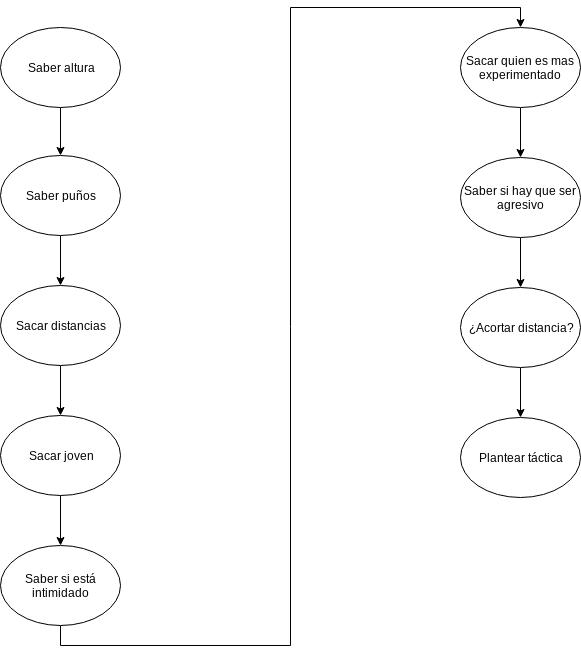
\includegraphics[width=0.8\linewidth]{mapaConocimiento1}
  \caption[Esquema toma decisión]{Esquema toma decisión}
  \label{fig:Esquema toma decisión anexo}
\end{figure}

\begin{figure}[htb]
  \centering
    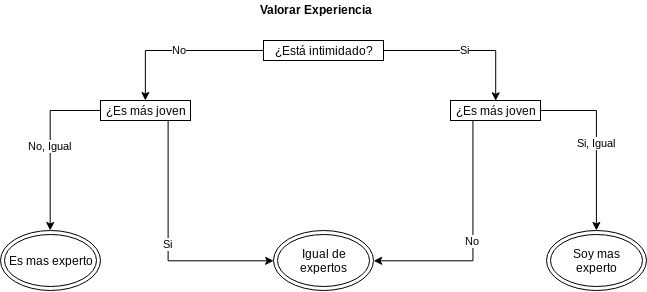
\includegraphics[width=0.8\linewidth]{MapaConocimientoExperiencia}
  \caption[Mapa de conocimiento experiencia]{Mapa de conocimiento experiencia}
  \label{fig:Arbol decisión experiencia anexo}
\end{figure}

\begin{figure}[htb]
  \centering
    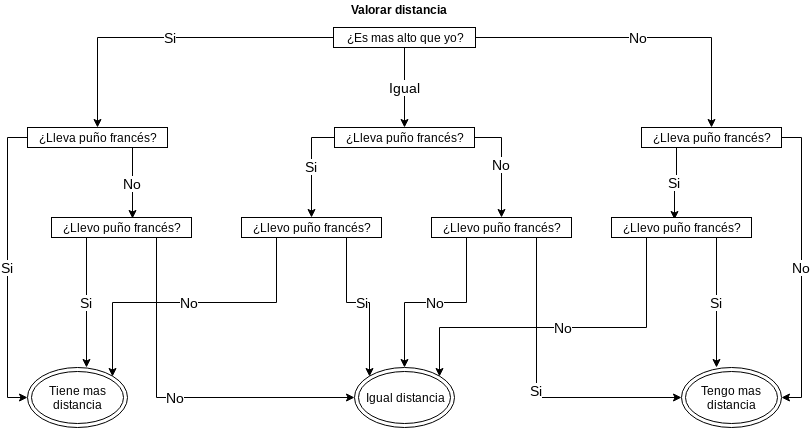
\includegraphics[width=0.8\linewidth]{MapaConocimientoDistancia}
  \caption[Mapa de conocimiento distancia]{Mapa de conocimiento distancia}
  \label{fig:Arbol decisión distancia anexo}
\end{figure}


\begin{figure}[htb]
  \centering
    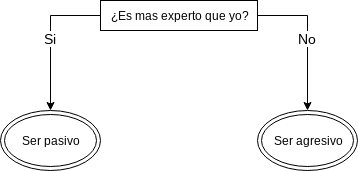
\includegraphics[width=0.8\linewidth]{MapaConocimientoAgresividad}
  \caption[Mapa de conocimiento agresividad]{Mapa de conocimiento agresividad}
  \label{fig:Arbol decisión agresividad anexo}
\end{figure}


\begin{figure}[htb]
  \centering
    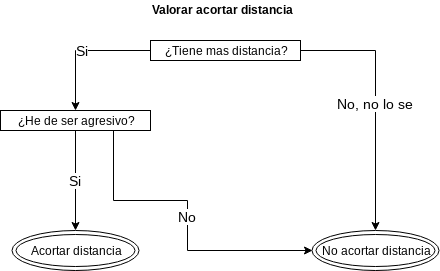
\includegraphics[width=0.8\linewidth]{MapaConocimientoAcortarDistancia}
  \caption[Mapa de conocimiento acortar distancia]{Mapa de conocimiento acortar distancia}
  \label{fig:Arbol decisión acortar distancia anexo}
\end{figure}


\begin{figure}[htb]
  \centering
    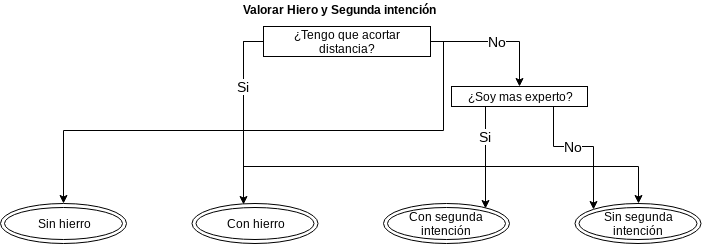
\includegraphics[width=0.8\linewidth]{MapaConocimientoHierroSIntencion}
  \caption[Mapa de conocimiento hierro y segunda intención]{Mapa de conocimiento hierro y segunda intención}
  \label{fig:Arbol decisión hierro y segunda intención anexo}
\end{figure}
 % Apéndice C (opcionales)

%---















%--- BACKMATTER
\backmatter
% -------------------------
%
% BIBLIOGRAFÍA
%
% -------------------------
% OJO: Todas las referencias deben estar citadas en el texto)
% EDITAR: Comentar línea siguiente
\nocite{*} % INCLUIDO para ver cómo queda, pero comentar en versión final.

\phantomsection  % OJO: Ojo necesario con hyperref.
\addcontentsline{toc}{chapter}{\bibname} % Añade la bibliografía al Índice de contenidos.
%---
% Opción 1: Bibliografía con todas las fuentes en un apartado.
%---
\printbibliography
%---

%---
% Opción 2: Bibliografía con secciones separadas.
%---
%\printbibheading
%\printbibliography[heading=subbibliography,type=online,title={Fuentes online}]
%\printbibliography[heading=subbibliography,nottype=online,title={Fuentes no online}]
% -------------------------
















% -------------------------
%
% ÍNDICE TEMÁTICO (opcional)
%
% -------------------------
% CONSEJO: Incluir los comandos mientras se escribe cada capítulo ya que hacerlo al final resulta tedioso.
\cleardoublepage
\phantomsection % OJO: Ojo necesario con hyperref.
\addcontentsline{toc}{chapter}{\indexname} % Añade al Índice de contenidos.

%---
% Impresión de Índice Temático (comentar para eliminar)
%---
\printindex  % Facilitado por makeidx (opcional, si no se usa no se imprime)

\end{document}
